\documentclass{article} % For LaTeX2e
\usepackage{iclr2016_conference,times}
\usepackage{hyperref}
\usepackage{url}
\usepackage{amsmath,amssymb,float}
\usepackage{multirow}
\usepackage{tabularx}
\usepackage{todonotes}
\usepackage{caption}
\usepackage{subcaption}
\DeclareMathOperator{\E}{\mathbb{E}}
\def\!#1{\boldsymbol{#1}}
\def\*#1{\mathbf{#1}}
\newcommand\independent{\protect\mathpalette{\protect\independenT}{\perp}}
\def\independenT#1#2{\mathrel{\rlap{$#1#2$}\mkern2mu{#1#2}}}


\title{The Variational Fair Autoencoder}
  
\author{Christos Louizos$^*$, Kevin Swersky$^\times$, Yujia Li$^\times$, Max Welling$^{*\dagger\ddagger}$, Richard Zemel$^{\times\dagger}$\\
	$^*$ Machine Learning Group, University of Amsterdam\\
	$^\times$Department of Computer Science, University of Toronto\\
	$^\dagger$ Canadian Institute for Advanced Research (CIFAR)\\
	$^\ddagger$ University of California, Irvine\\
	\texttt{C.Louizos@uva.nl, \{kswersky, yujiali\}@cs.toronto.edu}\\
	\texttt{M.Welling@uva.nl, zemel@cs.toronto.edu}}
	
\newcommand{\fix}{\marginpar{FIX}}
\newcommand{\new}{\marginpar{NEW}}

\iclrfinalcopy % Uncomment for camera-ready version

\begin{document}

\maketitle

\begin{abstract}
We investigate the problem of learning representations that are invariant to certain nuisance or sensitive factors of variation in the data while retaining as much of the remaining information as possible. Our model is based on a variational autoencoding architecture~\citep{kingma2013auto, rezende2014stochastic} with priors that encourage independence between sensitive and latent factors of variation. Any subsequent processing, such as classification, can then be performed on this purged latent representation. To remove any remaining dependencies we incorporate an additional penalty term based on the ``Maximum Mean Discrepancy'' (MMD)~\citep{gretton2006kernel} measure. We discuss how these architectures can be efficiently trained on data and show in experiments that this method is more effective than previous work in removing unwanted sources of variation while maintaining informative latent representations. 
\end{abstract}

\section{Introduction} 
In ``Representation Learning'' one tries to find representations of the data that are informative for a particular task while removing the factors of variation that are uninformative and are typically detrimental for the task under consideration. Uninformative dimensions are often called ``noise'' or ``nuisance variables'' while informative dimensions are usually called latent or hidden factors of variation. Many machine learning algorithms can be understood in this way: principal component analysis, nonlinear dimensional reduction and latent Dirichlet allocation are all models that extract informative factors (dimensions, causes, topics) of the data which can often be used to visualize the data. On the other hand, linear discriminant analysis and deep (convolutional) neural nets learn representations that are good for classification. 

In this paper we  consider the case where we wish to learn latent representations where (almost) all of the information about certain known factors of variation are purged from the representation while still retaining as much information about the data as possible. In other words, we want a latent representation $\*z$ that is maximally informative about an observed random variable $\*y$ (e.g., class label) while minimally informative about a \emph{sensitive} or \emph{nuisance} variable $\*s$. By treating $\*s$ as a sensitive variable, i.e. $\*s$ is correlated with our objective, we are dealing with ``fair representations'', a problem previously considered by~\cite{zemel2013learning}. If we instead treat $\*s$ as a nuisance variable we are dealing with ``domain adaptation'', in other words by removing the domain $\*s$ from our representations we will obtain \emph{improved} performance.

In this paper we introduce a novel model based on deep variational autoencoders (VAE)~\citep{kingma2013auto, rezende2014stochastic}. These models can naturally encourage separation between latent variables $\*z$ and sensitive variables $\*s$ by using factorized priors $p(\*s)p(\*z)$. However, some dependencies may still remain when mapping data-cases to their hidden representation using the variational posterior $q(\*z|\*x,\*s)$, which we stamp out using a ``Maximum Mean Discrepancy"~\citep{gretton2006kernel} term that penalizes differences between all order moments of the marginal posterior distributions $q(\*z|\*s=k)$ and $q(\*z|\*s=k')$ (for a discrete RV $\*s$). In experiments we show that this combined approach is highly successful in learning representations that are devoid of unwanted information while retaining as much information as possible from what remains. 

\section{Learning Invariant Representations}
\begin{figure}[ht]
    \begin{center}
        \begin{minipage}[b]{0.48\textwidth}
            \centering
            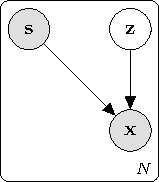
\includegraphics[scale=0.75]{unsupervised.pdf}
            \caption{Unsupervised model}
        \end{minipage}
        \quad
          \begin{minipage}[b]{0.48\textwidth}
            \centering
            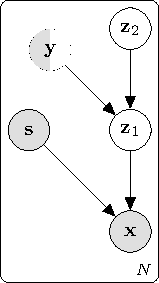
\includegraphics[scale=0.75]{semisupervised.pdf}
            \caption{Semi-supervised model}
        \end{minipage}
    \end{center}
\end{figure}

\subsection{Unsupervised model}
Factoring out undesired variations from the data can be easily formulated as a general probabilistic model which admits two distinct (independent) ``sources''; an observed variable $\*s$, which denotes the variations that we want to remove, and a continuous latent variable $\*z$ which models all the remaining information.  This generative process can be formally defined as:
\begin{align*}
	\*z \sim p(\*z); \qquad \*x \sim p_\theta(\*x| \*z, \*s)
\end{align*}
where $p_\theta(\*x| \*z, \*s)$ is an appropriate probability distribution for the data we are modelling. With this formulation we explicitly encode a notion of `invariance' in our model, since the latent representation is marginally independent of the factors of variation $\*s$. Therefore the problem of finding an invariant representation for a data point $\*x$ and variation $\*s$ can be cast as performing inference on this graphical model and obtaining the posterior distribution of $\*z$, $p(\*z|\*x, \*s)$. 

For our model we will employ a variational autoencoder architecture~\citep{kingma2013auto,rezende2014stochastic}; namely we will parametrize the generative model (decoder) $p_\theta(\*x|\*z,\*s)$ and  the variational posterior (encoder) $q_\phi(\*z|\*x,\*s)$ as (deep) neural networks which accept as inputs $\*z,\*s$ and $\*x,\*s$ respectively and produce the parameters of each distribution after a series of non-linear transformations. Both the model ($\theta$) and variational ($\phi$) parameters will be jointly optimized with the SGVB~\citep{kingma2013auto} algorithm according to a lower bound on the log-likelihood. This parametrization will allow us to capture most of the salient information of $\*x$ in our embedding $\*z$. Furthermore the distributed representation of a neural network would allow us to better resolve the dependencies between $\*x$ and $\*s$ thus yielding a better disentangling between the independent factors $\*z$ and $\*s$. By choosing a Gaussian posterior $q_\phi(\*z|\*x, \*s)$ and standard isotropic Gaussian prior $p(\*z) = \mathcal{N}(\*0, \*I)$ we can obtain the following lower bound:
\begin{align}
	\sum_{n=1}^{N}\log p(\*x_n|\*s_n) & \ge  \sum_{n=1}^{N}\E_{q_\phi(\*z_n|\*x_n,\*s_n)}[\log p_\theta(\*x_n|\*z_n,\*s_n)] - KL(q_\phi(\*z_n|\*x_n,\*s_n) || p(\*z))\\
	                    & = \mathcal{F}(\phi, \theta; \*x_n, \*s_n) \nonumber
\end{align}
with $q_\phi(\*z_n|\*x_n, \*s_n) = \mathcal{N}(\*z_n|\!\mu_n = f_\phi(\*x_n, \*s_n), \!\sigma_n = e^{f_\phi(\*x_n, \*s_n)})$ and $p_\theta(\*x_n|\*z_n, \*s_n) = f_\theta(\*z_n, \*s_n)$ with $f_\theta(\*z_n, \*s_n)$ being an appropriate probability distribution for the data we are modelling.

\subsection{Semi-Supervised model}
Factoring out variations in an unsupervised way can however be harmful in cases where we want to use this invariant representation for a subsequent prediction task. In particular if we have a situation where the nuisance variable $\*s$ and the actual label $\*y$ are correlated, then training an unsupervised model could yield \emph{random} or \emph{degenerate} representations with respect to $\*y$. Therefore it is more appropriate to try to ``inject'' the information about the label during the feature extraction phase. This can be quite simply achieved by introducing a second ``layer'' of latent variables to our generative model where we try to correlate $\*z$ with the prediction task. Assuming that the invariant features are now called $\*z_1$ we enrich the generative story by similarly providing two distinct (independent) sources for $\*z_1$; a discrete (in case of classification)variable $\*y$ which denotes the label of the data point $\*x$ and a continuous latent variable $\*z_2$ which encodes the variation on $\*z_1$ that is not explained by $\*y$ ($\*x$ dependent noise). The process now can be formally defined as: 
\begin{align*}
\*y, \*z_2 \sim \text{Cat}(\*y)p(\*z_2); \qquad  \*z_1 \sim p_\theta(\*z_1|\*z_2, \*y);\qquad \*x \sim p_\theta(\*x| \*z_1,\*s)\nonumber
\end{align*}   
Similarly to the unsupervised case we use a variational auto-encoder and jointly optimize the variational and model parameters. The lower bound now becomes:
\begin{align}
\sum_{n=1}^{N}\log p(\*x_n|\*s_n) & \ge \sum_{n=1}^{N}\E_{q_\phi({\*z_1}_n, {\*z_2}_n, \*y_n| \*x_n, \*s_n)}[\log p(\*z_2) + \log p(\*y_n) + \log p_\theta({\*z_1}_n|{\*z_2}_n, \*y_n) + \nonumber\\&\qquad\qquad\qquad\qquad + \log p_\theta(\*x_n|{\*z_1}_n,\*s_n) - \log q_\phi({\*z_1}_n, {\*z_2}_n, \*y_n|\*x_n, \*s_n)]  
\end{align}
where we assume that the posterior $q_\phi({\*z_1}_n, {\*z_2}_n, \*y_n|\*x_n, \*s_n)$ is factorized as $q_\phi({\*z_1}_n, {\*z_2}_n, \*y_n|\*x_n, \*s_n) = q_\phi({\*z_1}_n|\*x_n, \*s_n)q_\phi(\*y_n|{\*z_1}_n)q_\phi({\*z_2}_n|{\*z_1}_n,\*y_n)$, and where:
\begin{align*}
q_\phi({\*z_1}_n|\*x_n, \*s_n) & = \mathcal{N}({\*z_1}_n|\!\mu_n = f_\phi(\*x_n, \*s_n), \!\sigma_n = e^{f_\phi(\*x_n, \*s_n)}) \\
q_\phi(\*y_n | {\*z_1}_n) & = \text{Cat}(\*y_n|\!\pi_n = \text{softmax}(f_\phi({\*z_1}_n)))\\
q_\phi({\*z_2}_n|{\*z_1}_n, \*y_n) & = \mathcal{N}({\*z_2}_n| \!\mu_n = f_\phi({\*z_1}_n, \*y_n), \!\sigma_n = e^{f_\phi({\*z_1}_n, \*y_n)})\\
p_\theta({\*z_1}_n | {\*z_2}_n, \*y_n) & = \mathcal{N}({\*z_1}_n| \!\mu_n = f_\theta({\*z_2}_n, \*y_n), \!\sigma_n = e^{f_\theta({\*z_2}_n, \*y_n)})\\
p_\theta(\*x_n|{\*z_1}_n, \*s_n) & = f_\theta({\*z_1}_n, \*s_n)
\end{align*}
with $f_\theta({\*z_1}_n, \*s_n)$ again being an appropriate probability distribution for the data we are modelling. The model proposed here can be seen as an extension to the `stacked M1+M2' model originally proposed from~\cite{kingma2014semi}, where we have additionally introduced the nuisance variable $\*s$ during the feature extraction. Thus following~\cite{kingma2014semi} we can also handle the `semi-supervised' case, i.e., missing labels. In situations where the label is observed the lower bound takes the following form (exploiting the fact that we can compute some Kullback-Leibler divergences explicitly in our case):
\begin{align}
\sum_{n=1}^{N}\mathcal{L}_s(\phi, \theta; \*x_n, \*s_n, \*y_n) & =\sum_{n=1}^{N_s} \E_{q_\phi({\*z_1}_n|\*x_n, \*s_n)}[-KL(q_\phi({\*z_2}_n|{\*z_1}_n, \*y_n) || p(\*z_2)) + \log p_\theta(\*x_n|{\*z_1}_n, \*s_n)] +\nonumber\\&\qquad\qquad + \E_{q_\phi({\*z_1}_n|\*x_n, \*s_n)q_\phi({\*z_2}_n|{\*z_1}_n,\*y_n)}[\log p_\theta({\*z_1}|{\*z_2}_n, \*y_n)- \log q_\phi({\*z_1}_n|\*x_n \*s_n)]
\end{align}
and in the case that it is not observed we use $q(\*y_n|{\*z_1}_n)$ to `impute' our data:
\begin{align}
\sum_{m=1}^{M}\mathcal{L}_u(\phi, \theta; \*x_m, \*s_m) & = \sum_{m=1}^{M}\E_{q_\phi({\*z_1}_m|\*x_m,\*s_m)}[ - KL (q(\*y_m|{\*z_1}_m) || p(\*y_m)) + \log p_\theta(\*x_m|{\*z_1}_m, \*s_m)] +\nonumber\\&\qquad\qquad +  \E_{q_\phi({\*z_1}_m, \*y_m|\*x_m,\*s_m)}[ - KL (q_\phi({\*z_2}_m|{\*z_1}_m,\*y_m) || p(\*z_2))] +\nonumber\\&\qquad\qquad+  \E_{q_\phi({\*z_1}_m, \*y_m, {\*z_2}_m|\*x_m, \*s_m)}[\log p_\theta({\*z_1}_m|{\*z_2}_m,\*y_m) -\log q_\phi({\*z_1}_m|\*x_m,\*s_m) ]
\end{align}
therefore the final objective function is:
\begin{align}
    \mathcal{F}_{\text{VAE}}(\phi, \theta; \*x_n, \*x_m, \*s_n, \*s_m, \*y_n) & = \sum_{n=1}^{N}\mathcal{L}_s(\phi, \theta; \*x_n, \*s_n, \*y_n) + \sum_{m=1}^{M}\mathcal{L}_u(\phi, \theta; \*x_m, \*s_m) + \nonumber \\ &\qquad\qquad +  \alpha\sum_{n=1}^{N}\E_{q({\*z_1}_n|\*x_n, \*s_n)}[- \log q_\phi(\*y_n|{\*z_1}_n)]
\end{align}
where the last term is introduced so as to ensure that the predictive posterior $q_\phi(\*y|\*z_1)$ learns from both labeled and unlabeled data. This semi-supervised model will be called ``VAE'' in our experiments.

However, there is a subtle difference between the approach of~\cite{kingma2014semi} and our model. Instead of training separately each layer of stochastic variables we optimize the model jointly. The potential advantages of this approach are two fold: as we previously mentioned if the label $\*y$ and the nuisance information $\*s$ are correlated then training a (conditional) feature extractor separately poses the danger of creating a degenerate representation with respect to the label $\*y$. Furthermore the label information will also better guide the feature extraction towards the more salient parts of the data, thus maintaining most of the (predictive) information.


\subsection{Further invariance via Maximum Mean Discrepancy}
Despite the fact that we have a model that encourages statistical independence between $\*s$ and $\*z_1$ a-priori we might still have some dependence in the (approximate) marginal posterior $q_{\phi}(\*z_1|\*s)$. In particular, this can happen if the label $\*y$ is correlated with the sensitive variable $\*s$, which can allow information about $\*s$ to ``leak'' into the posterior. Thus instead we could maximize a ``penalized'' lower bound where we impose some sort of regularization on the marginal $q_{\phi}(\*z_1|\*s)$. In the following we will describe one way to achieve this regularization through the Maximum Mean Discrepancy (MMD)~\citep{gretton2006kernel} measure.

 
\subsubsection{Maximum Mean Discrepancy}
Consider the problem of determining whether two datasets $\{ \*X \} \sim P_0$ and $\{ \*X' \} \sim P_1$ are drawn from the same distribution, i.e., $P_0 = P_1$. A simple test is to consider the distance between empirical statistics $\psi(\cdot)$ of the two datasets:
\begin{equation}
    \left \| \frac{1}{N_0} \sum_{i=1}^{N_0} \psi(\*x_i) - \frac{1}{N_1} \sum_{i=1}^{N_1} \psi(\*x'_i) \right \|^2. \label{eq:premmd}
\end{equation}
Expanding the square yields an estimator composed only of inner products on which the kernel trick can be applied. The resulting estimator is known as Maximum Mean Discrepancy (MMD)~\citep{gretton2006kernel}:
\begin{align}
    \ell_{\mathrm{MMD}}(\*X, \*X') &= \frac{1}{N_0^2} \sum_{n=1}^{N_0} \sum_{m=1}^{N_0} k(\*x_n, \*x_{m}) + \frac{1}{N_1^2} \sum_{n=1}^{N_1} \sum_{m=1}^{N_1} k(\*x'_n, \*x'_m) - \frac{2}{N_0 N_1} \sum_{n=1}^{N_0} \sum_{m=1}^{N_1} k(\*x_n, \*x'_m). \label{eq:mmd}
\end{align}
Asymptotically, for a universal kernel such as the Gaussian kernel $k(x,x')=e^{-\gamma \| \*x - \*x' \|^2}$, $\ell_{\mathrm{MMD}}(\*X, \*X')$ is $0$ if and only if $P_0 = P_1$. Equivalently, minimizing MMD can be viewed as matching all of the moments of $P_0$ and $P_1$.  Therefore, we can use it as an extra ``regularizer'' and force the model to try to match the moments between the marginal posterior distributions of our latent variables, i.e., $q_{\phi}(\*z_1|s=0)$ and $q_{\phi}(\*z_1| s=1)$ (in the case of binary nuisance information $\*s$\footnote{In case that we have more than two states for the nuisance information $\*s$, we minimize the MMD penalty between each marginal $q(\*z|\*s=k)$ and $q(\*z)$, i.e., $\sum_{k=1}^{K}\ell_{\mathrm{MMD}}({\*Z_1}_{\*s=k}, {\*Z_1})$ for all possible states $K$ of $\*s$.}). By adding the MMD penalty into the lower bound of our aforementioned VAE architecture we obtain our proposed model, the ``Variational Fair Autoencoder'' (VFAE):
\begin{align}
    \mathcal{F}_{\text{VFAE}}(\phi, \theta; \*x_n, \*x_m, \*s_n, \*s_m, \*y_n) & = \mathcal{F}_{\text{VAE}}(\phi, \theta; \*x_n, \*x_m, \*s_n, \*s_m, \*y_n) -\beta \ell_{\mathrm{MMD}}({\*Z_1}_{\*s=0}, {\*Z_1}_{\*s=1})
\end{align}
where:
\begin{align}
  \ell_{\mathrm{MMD}}({\*Z_1}_{\*s=0}, {\*Z_1}_{\*s=1}) & = \|\E_{\tilde{p}(\*x|\*s=0)}[\E_{q(\*z_1|\*x, \*s=0)}[\psi(\*z_1)]] - E_{\tilde{p}(\*x|\*s=1)}[\E_{q(\*z_1|\*x, \*s=1)}[\psi(\*z_1)]]\|^2
\end{align}

\subsection{Fast MMD via Random Fourier Features}
A naive implementation of MMD in minibatch stochastic gradient descent would require computing the $M\times M$ Gram matrix for each minibatch during training, where $M$ is the minibatch size. Instead, we can use random kitchen sinks~\citep{rahimi2009weighted} to compute a feature expansion such that computing the estimator $(\ref{eq:premmd})$ approximates the full MMD (\ref{eq:mmd}). To compute this, we draw a random $K\times D$ matrix $\*W$, where $K$ is the dimensionality of $\*x$, $D$ is the number of random features and each entry of $\*W$ is drawn from a standard isotropic Gaussian.
The feature expansion is then given as:
\begin{align}
\psi_\*W(\*x) &= \sqrt{\frac{2}{D}}\mathrm{cos}\left ( \sqrt{\frac{2}{\gamma}} \*x\*W + \*b \right ).
\end{align}
where $\*b$ is a $D$-dimensional uniform random vector with entries in $[0,2\pi]$. \cite{zhao2014fastmmd} have successfully applied the idea of using random kitchen sinks to approximate MMD. This estimator is fairly accurate, and is typically much faster than the full MMD penalty. We use $D=500$ in our experiments.


\section{Experiments}
\section{Experiments}
\label{sect:experiments}

% \begin{figure*}
%   \centering
%   \setlength{\tabcolsep}{0pt}
%   \setlength\figurewidth{0.05\textwidth}
%   \newcommand{\example}[1]{\raisebox{-.4\height}{\includegraphics[width=\figurewidth]{./figures/domains_examples/#1}}}
%   \begin{sc}
%   \begin{tabular}{r@{\hskip 1cm} ccccccccccc}
%     MNIST \cite{LeCun98} &
%     \example{mnist_0.png} &
%     \example{mnist_1.png} &
%     \example{mnist_2.png} &
%     \example{mnist_3.png} &
%     \example{mnist_4.png} &
%     \example{mnist_5.png} &
%     \example{mnist_6.png} &
%     \example{mnist_7.png} &
%     \example{mnist_8.png} &
%     \example{mnist_9.png} &
%     \example{mnist_10.png}\\
%     MNIST ($ | \Delta | $, BG) &
%     \example{mnisti_0.png} &
%     \example{mnisti_1.png} &
%     \example{mnisti_2.png} &
%     \example{mnisti_3.png} &
%     \example{mnisti_4.png} &
%     \example{mnisti_5.png} &
%     \example{mnisti_6.png} &
%     \example{mnisti_7.png} &
%     \example{mnisti_8.png} &
%     \example{mnisti_9.png} &
%     \example{mnisti_10.png}\\
%     Syn Numbers &
%     \example{syn_0.png} &
%     \example{syn_1.png} &
%     \example{syn_2.png} &
%     \example{syn_3.png} &
%     \example{syn_4.png} &
%     \example{syn_5.png} &
%     \example{syn_6.png} &
%     \example{syn_7.png} &
%     \example{syn_8.png} &
%     \example{syn_9.png} &
%     \example{syn_10.png}\\
%     SVHN \cite{Netzer11} &
%     \example{svhn_0.png} &
%     \example{svhn_1.png} &
%     \example{svhn_2.png} &
%     \example{svhn_3.png} &
%     \example{svhn_4.png} &
%     \example{svhn_5.png} &
%     \example{svhn_6.png} &
%     \example{svhn_7.png} &
%     \example{svhn_8.png} &
%     \example{svhn_9.png} &
%     \example{svhn_10.png}\\
%     Syn Signs &
%     \example{synsgn_11.png} &
%     \example{synsgn_1.png} &
%     \example{synsgn_2.png} &
%     \example{synsgn_3.png} &
%     \example{synsgn_4.png} &
%     \example{synsgn_5.png} &
%     \example{synsgn_12.png} &
%     \example{synsgn_7.png} &
%     \example{synsgn_8.png} &
%     \example{synsgn_9.png} &
%     \example{synsgn_10.png}\\
%     GTSRB \cite{Stallkamp12} &
%     \example{gtsrb_0.png} &
%     \example{gtsrb_1.png} &
%     \example{gtsrb_2.png} &
%     \example{gtsrb_3.png} &
%     \example{gtsrb_4.png} &
%     \example{gtsrb_5.png} &
%     \example{gtsrb_6.png} &
%     \example{gtsrb_7.png} &
%     \example{gtsrb_8.png} &
%     \example{gtsrb_9.png} &
%     \example{gtsrb_10.png}\\
%     % CIFAR-10 \cite{Krizhevsky09} &
%     % \example{cifar10_0.png} &
%     % \example{cifar10_1.png} &
%     % \example{cifar10_2.png} &
%     % \example{cifar10_3.png} &
%     % \example{cifar10_4.png} &
%     % \example{cifar10_5.png} &
%     % \example{cifar10_11.png} &
%     % \example{cifar10_7.png} &
%     % \example{cifar10_8.png} &
%     % \example{cifar10_9.png} &
%     % \example{cifar10_10.png}\\
%     % STL-10 \cite{Coates11} &
%     % \example{stl10_12.png} &
%     % \example{stl10_1.png} &
%     % \example{stl10_2.png} &
%     % \example{stl10_3.png} &
%     % \example{stl10_4.png} &
%     % \example{stl10_5.png} &
%     % \example{stl10_6.png} &
%     % \example{stl10_13.png} &
%     % \example{stl10_8.png} &
%     % \example{stl10_9.png} &
%     % \example{stl10_10.png}\\
%   \end{tabular}
%   \end{sc}
%   \vskip 2.5mm
%   \caption{\todo[What to do with this figure? Add Office? Remove?]Random samples from the datasets used in the experiments. See \sect{exper_quant} for details.}
%   \label{fig:exper_domains_examples}
% \end{figure*}

\begin{figure*}
  \centering
  \setlength{\tabcolsep}{0pt}
  \setlength\figurewidth{0.05\textwidth}
  \newcommand{\example}[1]{\raisebox{-.4\height}{\includegraphics[width=\figurewidth]{./figures/domains_examples/#1}}}
  \begin{sc}
  \begin{small}
  \begin{tabular}{r@{\hskip 0.5cm} ccc c@{\hskip 0.4cm} ccc c@{\hskip 0.4cm} ccc c@{\hskip 0.4cm} ccc}
    &
    \multicolumn{3}{c}{MNIST} & &
    \multicolumn{3}{c}{Syn Numbers} & &
    \multicolumn{3}{c}{SVHN} & &
    \multicolumn{3}{c}{Syn Signs}\\
    
    Source &
    \example{mnist_0.png} &
    \example{mnist_1.png} &
    \example{mnist_3.png} & &
    
    \example{syn_0.png} &
    \example{syn_1.png} &
    \example{syn_2.png} & &
    
    \example{svhn_3.png} &
    \example{svhn_4.png} &
    \example{svhn_5.png} & &
    
    \example{synsgn_3.png} &
    \example{synsgn_4.png} &
    \example{synsgn_5.png}\\
    
    Target &
    \example{mnisti_0.png} &
    \example{mnisti_1.png} &
    \example{mnisti_2.png} & &
    
    \example{svhn_0.png} &
    \example{svhn_1.png} &
    \example{svhn_2.png} & &
    
    \example{mnist_4.png} &
    \example{mnist_5.png} &
    \example{mnist_6.png} & &
    
    \example{gtsrb_2.png} &
    \example{gtsrb_3.png} &
    \example{gtsrb_4.png}\\
    
    &
    \multicolumn{3}{c}{\rule{0pt}{0.35cm} MNIST-M} & &
    \multicolumn{3}{c}{SVHN} & &
    \multicolumn{3}{c}{MNIST} & &
    \multicolumn{3}{c}{GTSRB}\\
  \end{tabular}
  \end{small}
  \end{sc}
  \caption{Examples of domain pairs used in the experiments. See \sect{exper_quant} for details.}
  \label{fig:exper_domains_examples}
\end{figure*}


\begin{table*}[t]
  \vskip 0.15in
  \begin{center}
    \begin{small}
      \begin{sc}
        \renewcommand{\arraystretch}{1.5}
        \begin{tabular}{l r | c c c c}
          \hline
          \multirow{2}{*}{Method} & {\scriptsize Source} & MNIST & Syn Numbers & SVHN & Syn Signs \\
          & {\scriptsize Target} & MNIST-M & SVHN & MNIST & GTSRB \\
          \hline
          \multicolumn{2}{l |}{Source only} & 
          $ .5749 $                      & $ .8665 $                      & $ .5919 $                      & $ .7400 $                      \\
          \multicolumn{2}{l |}{SA \cite{Fernando13}} & 
          $ .6078 \; (7.9\%) $           & $ .8672 \; (1.3\%) $           & $ .6157 \; (5.9\%) $           & $ .7635 \; (9.1\%) $           \\
          \multicolumn{2}{l |}{Proposed approach} & 
          $ \mathbf{.8149} \; (57.9\%) $ & $ \mathbf{.9048} \; (66.1\%) $ & $ \mathbf{.7107} \; (29.3\%) $ & $ \mathbf{.8866} \; (56.7\%) $ \\
          \multicolumn{2}{l |}{Train on target} & 
          $ .9891 $                      & $ .9244 $                      & $ .9951 $                      & $ .9987 $                      \\
          \hline
        \end{tabular}
      \end{sc}
    \end{small}
  \end{center}
    \caption{Classification accuracies for digit image classifications for different source and target domains. {\sc MNIST-M} corresponds to difference-blended digits over non-uniform background. The first row corresponds to the lower performance bound (i.e.\ if no adaptation is performed). The last row corresponds to training on the target domain data with known class labels (upper bound on the DA performance). For each of the two DA methods (ours and \cite{Fernando13}) we show how much of the gap between the lower and the upper bounds was covered (in brackets). For all five cases, our approach outperforms \cite{Fernando13} considerably, and covers a big portion of the gap.\vspace{-0mm} }
  \label{tab:results}
  \vskip -0.1in
\end{table*}

\begin{table*}[t]
  \vskip 0.15in
  \begin{center}
    \begin{small}
      \begin{sc}
        \renewcommand{\arraystretch}{1.5}
        \begin{tabular}{l r | c c c}
          \hline
          \multirow{2}{*}{Method} & {\scriptsize Source} & Amazon & DSLR & Webcam \\
          & {\scriptsize Target} & Webcam & Webcam & DSLR \\
          \hline
          \multicolumn{2}{l |}{GFK(PLS, PCA) \cite{Gong12}} & 
          $ .464 \pm .005 $ & $ .613 \pm .004 $ & $ .663 \pm .004 $\\ 
          \multicolumn{2}{l |}{SA \cite{Fernando13}} & 
          $ .450 $ & $ .648 $ & $ .699 $\\ 
          \multicolumn{2}{l |}{DA-NBNN \cite{Tommasi13}} & 
          $ .528 \pm .037 $ & $ .766 \pm .017 $ & $ .762 \pm .025 $\\ 
          \multicolumn{2}{l |}{DLID \cite{Chopra13}} & 
          $ .519 $ & $ .782 $ & $ .899 $\\
          \multicolumn{2}{l |}{DeCAF$_6$ Source Only \cite{Donahue14}} &
          $ .522 \pm .017 $ & $ .915 \pm .015 $ & --\\ 
          \multicolumn{2}{l |}{DaNN \cite{Ghifary14}} & 
          $ .536 \pm .002 $ & $ .712 \pm .000 $ & $ .835 \pm .000 $\\ 
          \multicolumn{2}{l |}{DDC \cite{Tzeng14}} & 
          $ .594 \pm .008 $ & $ .925 \pm .003 $ & $ .917 \pm .008 $\\ 
          \multicolumn{2}{l |}{Proposed Approach} & 
          $ \mathbf{ .673 \pm .017 } $ & $ \mathbf{ .940 \pm .008 } $ & $ \mathbf{ .937 \pm .010 } $\\
          \hline
        \end{tabular}
      \end{sc}
    \end{small}
  \end{center}
    \caption{Accuracy evaluation of different DA approaches on the standard {\sc Office} \cite{Saenko10} dataset. Our method (last row) outperforms competitors setting the new state-of-the-art.}
  \label{tab:results_office}
\end{table*}

% Other rows refer to the following algorithms (from top to bottom): Geodesic Flow Kernel \cite{Gong12}, Subspace Alignment \cite{Fernando13}, Naive Bayes Nearest Neighbor \cite{Tommasi13},  deep learning approach from \cite{Chopra13}, DeCAF$_6$-features described in \cite{Donahue14}, Domain Adaptive NNs \cite{Ghifary14}, Deep Domain Confusion \cite{Tzeng14}.

\def\X{{\mathbf X}}
\def\y{{\mathbf y}}

% \vspace{2mm}\noindent {\bf Datasets.}
% \label{sect:exper_datasets}

% In order to test our method in the setting of traffic signs classification we obtained~100,000 synthetic images ({\sc Syn~Signs}) simulating various photoshooting conditions. This dataset was used in conjunction with {\it The German Traffic Sign Recognition Benchmark} ({\sc GTSRB}) \cite{Stallkamp12}.

% Finally, we perform domain adaption for the {\sc CIFAR-10} and the {\sc STL-10} downsampled to the size of $ 32 \times 32 $. This pair is considerably different from the previously mentioned datasets as the intra-class variability here is higher.

We perform extensive evaluation of the proposed approach on a number of popular image datasets and their modifications. These include large-scale datasets of small images popular with deep learning methods, and the {\sc Office} datasets \cite{Saenko10}, which are a {\em de facto} standard for domain adaptation in computer vision, but have much fewer images.

\vspace{2mm}\noindent {\bf Baselines.} For the bulk of experiments the following baselines are evaluated. The \textbf{source-only} model is trained without consideration for target-domain data (no domain classifier branch included into the network). The \textbf{train-on-target} model is trained on the target domain with class labels revealed. This model serves as an upper bound on DA methods, assuming that target data are abundant and the shift between the domains is considerable. 

In addition, we compare our approach against the recently proposed unsupervised DA method based on \textbf{subspace alignment (SA)} \cite{Fernando13}, which is simple to setup and test on new datasets, but has also been shown to perform very well in experimental comparisons with other ``shallow'' DA methods. To boost the performance of this baseline, we pick its most important free parameter (the number of principal components) from the range $ \{ 2, \ldots, 60 \} $, so that the test performance on the target domain is maximized. To apply SA in our setting, we train a source-only model and then consider the activations of the last hidden layer in the label predictor (before the final linear classifier) as descriptors/features, and learn the mapping between the source and the target domains \cite{Fernando13}.

Since the SA baseline requires to train a new classifier after adapting the features, and in order to put all the compared settings on an equal footing, we retrain the last layer of the label predictor using a standard linear SVM~\cite{liblinear} for all four considered methods (including ours; the performance on the target domain remains approximately the same after the retraining). 

For the {\sc Office} dataset \cite{Saenko10}, we directly compare the performance of our full network (feature extractor and label predictor) against recent DA approaches using previously published results.

\vspace{2mm}\noindent {\bf CNN architectures.} In general, we compose feature extractor from two or three convolutional layers, picking their exact configurations from previous works. We give the exact architectures in \ref{sect:appendix_archs}.

For the domain adaptator we stick to the three fully connected layers ($x\rightarrow1024\rightarrow1024\rightarrow2$), except for {\sc MNIST} where we used a simpler ($x\rightarrow100\rightarrow2$) architecture to speed up the experiments.

For loss functions, we set $ L_y $ and $ L_d $ to be the logistic regression loss and the binomial cross-entropy respectively.

\vspace{2mm}\noindent {\bf CNN training procedure.}
The model is trained on $128$-sized batches. Images are preprocessed by the mean subtraction. A half of each batch is populated by the samples from the source domain (with known labels), the rest is comprised of the target domain (with unknown labels).

In order to suppress noisy signal from the domain classifier at the early stages of the training procedure instead of fixing the adaptation factor $ \lambda $, we gradually change it from $0$ to $1$ using the following schedule:
\begin{equation}
  \lambda_p = \frac{2}{1 + \exp(-\gamma \cdot p)} - 1,
\end{equation}
where $\gamma$ was set to $10$ in all experiments (the schedule was not optimized/tweaked). Further details on the CNN training can be found in \ref{sect:appendix_training}.

\vspace{2mm}\noindent {\bf Visualizations.}
We use t-SNE \cite{Maaten13} projection to visualize feature distributions at different points of the network, while color-coding the domains (\fig{exper_adapt_vis}). We observe strong correspondence between the success of the adaptation in terms of the classification accuracy for the target domain, and the overlap between the domain distributions in such visualizations.
 
\vspace{2mm}\noindent {\bf Choosing meta-parameters.} 
In general, good unsupervised DA methods should provide ways to set meta-parameters (such as $\lambda$, the learning rate, the momentum rate, the network architecture for our method) in an unsupervised way, i.e.\ without referring to labeled data in the target domain. %Here we would like to give few recommendations concerning this matter. First, as it was pointed out in \sect{theory} the domain classifier should not be significantly more complex than the label predictor. 
In our method, one can assess the performance of the whole system (and the effect of changing hyper-parameters) by observing the test error on the source domain {\em and} the domain classifier error. In general, we observed a good correspondence between the success of adaptation and these errors (adaptation is more successful when the source domain test error is low, while the domain classifier error is high).
In addition, the layer, where the the domain adaptator is attached can be picked by computing difference between means as suggested in \cite{Tzeng14}. 

% \begin{figure*}
%   \centering
%   {\sc MNIST $ \rightarrow $ MNIST ($ | \Delta | $, bg)}: top feature extractor layer
%   \setcounter{subfigure}{0}
%   \subfigure[Non-adapted]{%%
%     \scalebox{0.8}{%% Creator: Matplotlib, PGF backend
%%
%% To include the figure in your LaTeX document, write
%%   \input{<filename>.pgf}
%%
%% Make sure the required packages are loaded in your preamble
%%   \usepackage{pgf}
%%
%% Figures using additional raster images can only be included by \input if
%% they are in the same directory as the main LaTeX file. For loading figures
%% from other directories you can use the `import` package
%%   \usepackage{import}
%% and then include the figures with
%%   \import{<path to file>}{<filename>.pgf}
%%
%% Matplotlib used the following preamble
%%   \usepackage[utf8x]{inputenc}
%%   \usepackage[T1]{fontenc}
%%
\begingroup%
\makeatletter%
\begin{pgfpicture}%
\pgfpathrectangle{\pgfpointorigin}{\pgfqpoint{3.338520in}{2.040000in}}%
\pgfusepath{use as bounding box}%
\begin{pgfscope}%
\pgfsetbuttcap%
\pgfsetroundjoin%
\definecolor{currentfill}{rgb}{1.000000,1.000000,1.000000}%
\pgfsetfillcolor{currentfill}%
\pgfsetlinewidth{0.000000pt}%
\definecolor{currentstroke}{rgb}{1.000000,1.000000,1.000000}%
\pgfsetstrokecolor{currentstroke}%
\pgfsetdash{}{0pt}%
\pgfpathmoveto{\pgfqpoint{0.000000in}{-0.000000in}}%
\pgfpathlineto{\pgfqpoint{3.338520in}{-0.000000in}}%
\pgfpathlineto{\pgfqpoint{3.338520in}{2.040000in}}%
\pgfpathlineto{\pgfqpoint{0.000000in}{2.040000in}}%
\pgfpathclose%
\pgfusepath{fill}%
\end{pgfscope}%
\begin{pgfscope}%
\pgftext[at=\pgfqpoint{0.510000in}{0.348333in},left,bottom]{\pgfimage[interpolate=true,width=2.553333in,height=1.500000in]{./figures/adaptation_vis/pool2_mnist2inv_before-img0.png}}%
\end{pgfscope}%
\begin{pgfscope}%
\pgftext[at=\pgfqpoint{0.805000in}{0.383333in},left,bottom]{\pgfimage[interpolate=true,width=2.201667in,height=1.371667in]{./figures/adaptation_vis/pool2_mnist2inv_before-img1.png}}%
\end{pgfscope}%
\end{pgfpicture}%
\makeatother%
\endgroup%
}}%%
%   \subfigure[Adapted]{%%
%     \scalebox{0.8}{%% Creator: Matplotlib, PGF backend
%%
%% To include the figure in your LaTeX document, write
%%   \input{<filename>.pgf}
%%
%% Make sure the required packages are loaded in your preamble
%%   \usepackage{pgf}
%%
%% Figures using additional raster images can only be included by \input if
%% they are in the same directory as the main LaTeX file. For loading figures
%% from other directories you can use the `import` package
%%   \usepackage{import}
%% and then include the figures with
%%   \import{<path to file>}{<filename>.pgf}
%%
%% Matplotlib used the following preamble
%%   \usepackage[utf8x]{inputenc}
%%   \usepackage[T1]{fontenc}
%%
\begingroup%
\makeatletter%
\begin{pgfpicture}%
\pgfpathrectangle{\pgfpointorigin}{\pgfqpoint{3.340000in}{2.040000in}}%
\pgfusepath{use as bounding box}%
\begin{pgfscope}%
\pgfsetbuttcap%
\pgfsetroundjoin%
\definecolor{currentfill}{rgb}{1.000000,1.000000,1.000000}%
\pgfsetfillcolor{currentfill}%
\pgfsetlinewidth{0.000000pt}%
\definecolor{currentstroke}{rgb}{1.000000,1.000000,1.000000}%
\pgfsetstrokecolor{currentstroke}%
\pgfsetdash{}{0pt}%
\pgfpathmoveto{\pgfqpoint{0.000000in}{-0.000000in}}%
\pgfpathlineto{\pgfqpoint{3.340000in}{-0.000000in}}%
\pgfpathlineto{\pgfqpoint{3.340000in}{2.040000in}}%
\pgfpathlineto{\pgfqpoint{0.000000in}{2.040000in}}%
\pgfpathclose%
\pgfusepath{fill}%
\end{pgfscope}%
\begin{pgfscope}%
\pgftext[at=\pgfqpoint{0.518333in}{0.321667in},left,bottom]{\pgfimage[interpolate=true,width=2.565000in,height=1.550000in]{./figures/adaptation_vis/pool2_mnist2inv_after-img0.png}}%
\end{pgfscope}%
\begin{pgfscope}%
\pgftext[at=\pgfqpoint{0.518333in}{0.321667in},left,bottom]{\pgfimage[interpolate=true,width=2.565000in,height=1.553333in]{./figures/adaptation_vis/pool2_mnist2inv_after-img1.png}}%
\end{pgfscope}%
\end{pgfpicture}%
\makeatother%
\endgroup%
}}\\
%   \vspace{5mm}
%   {\sc Syn Numbers $ \rightarrow $ SVHN}: last hidden layer of the label predictor
%   \setcounter{subfigure}{0}
%   \subfigure[Non-adapted]{%%
%     \scalebox{0.8}{%% Creator: Matplotlib, PGF backend
%%
%% To include the figure in your LaTeX document, write
%%   \input{<filename>.pgf}
%%
%% Make sure the required packages are loaded in your preamble
%%   \usepackage{pgf}
%%
%% Figures using additional raster images can only be included by \input if
%% they are in the same directory as the main LaTeX file. For loading figures
%% from other directories you can use the `import` package
%%   \usepackage{import}
%% and then include the figures with
%%   \import{<path to file>}{<filename>.pgf}
%%
%% Matplotlib used the following preamble
%%   \usepackage[utf8x]{inputenc}
%%   \usepackage[T1]{fontenc}
%%
\begingroup%
\makeatletter%
\begin{pgfpicture}%
\pgfpathrectangle{\pgfpointorigin}{\pgfqpoint{3.340000in}{2.040000in}}%
\pgfusepath{use as bounding box}%
\begin{pgfscope}%
\pgfsetbuttcap%
\pgfsetroundjoin%
\definecolor{currentfill}{rgb}{1.000000,1.000000,1.000000}%
\pgfsetfillcolor{currentfill}%
\pgfsetlinewidth{0.000000pt}%
\definecolor{currentstroke}{rgb}{1.000000,1.000000,1.000000}%
\pgfsetstrokecolor{currentstroke}%
\pgfsetdash{}{0pt}%
\pgfpathmoveto{\pgfqpoint{0.000000in}{-0.000000in}}%
\pgfpathlineto{\pgfqpoint{3.340000in}{-0.000000in}}%
\pgfpathlineto{\pgfqpoint{3.340000in}{2.040000in}}%
\pgfpathlineto{\pgfqpoint{0.000000in}{2.040000in}}%
\pgfpathclose%
\pgfusepath{fill}%
\end{pgfscope}%
\begin{pgfscope}%
\pgftext[at=\pgfqpoint{0.491667in}{0.335000in},left,bottom]{\pgfimage[interpolate=true,width=2.618333in,height=1.531667in]{./figures/adaptation_vis/before-img0.png}}%
\end{pgfscope}%
\begin{pgfscope}%
\pgftext[at=\pgfqpoint{0.758333in}{0.331667in},left,bottom]{\pgfimage[interpolate=true,width=2.171667in,height=1.436667in]{./figures/adaptation_vis/before-img1.png}}%
\end{pgfscope}%
\begin{pgfscope}%
\pgfsetbuttcap%
\pgfsetroundjoin%
\definecolor{currentfill}{rgb}{0.000000,0.000000,1.000000}%
\pgfsetfillcolor{currentfill}%
\pgfsetfillopacity{0.300000}%
\pgfsetlinewidth{0.150562pt}%
\definecolor{currentstroke}{rgb}{0.000000,0.000000,0.000000}%
\pgfsetstrokecolor{currentstroke}%
\pgfsetstrokeopacity{0.300000}%
\pgfsetdash{}{0pt}%
\pgfpathmoveto{\pgfqpoint{2.521160in}{1.775861in}}%
\pgfpathcurveto{\pgfqpoint{2.525278in}{1.775861in}}{\pgfqpoint{2.529228in}{1.777497in}}{\pgfqpoint{2.532140in}{1.780409in}}%
\pgfpathcurveto{\pgfqpoint{2.535052in}{1.783321in}}{\pgfqpoint{2.536688in}{1.787271in}}{\pgfqpoint{2.536688in}{1.791389in}}%
\pgfpathcurveto{\pgfqpoint{2.536688in}{1.795507in}}{\pgfqpoint{2.535052in}{1.799457in}}{\pgfqpoint{2.532140in}{1.802369in}}%
\pgfpathcurveto{\pgfqpoint{2.529228in}{1.805281in}}{\pgfqpoint{2.525278in}{1.806917in}}{\pgfqpoint{2.521160in}{1.806917in}}%
\pgfpathcurveto{\pgfqpoint{2.517042in}{1.806917in}}{\pgfqpoint{2.513092in}{1.805281in}}{\pgfqpoint{2.510180in}{1.802369in}}%
\pgfpathcurveto{\pgfqpoint{2.507268in}{1.799457in}}{\pgfqpoint{2.505631in}{1.795507in}}{\pgfqpoint{2.505631in}{1.791389in}}%
\pgfpathcurveto{\pgfqpoint{2.505631in}{1.787271in}}{\pgfqpoint{2.507268in}{1.783321in}}{\pgfqpoint{2.510180in}{1.780409in}}%
\pgfpathcurveto{\pgfqpoint{2.513092in}{1.777497in}}{\pgfqpoint{2.517042in}{1.775861in}}{\pgfqpoint{2.521160in}{1.775861in}}%
\pgfpathclose%
\pgfusepath{stroke,fill}%
\end{pgfscope}%
\begin{pgfscope}%
\pgfsetbuttcap%
\pgfsetroundjoin%
\definecolor{currentfill}{rgb}{0.000000,0.000000,1.000000}%
\pgfsetfillcolor{currentfill}%
\pgfsetfillopacity{0.300000}%
\pgfsetlinewidth{0.150562pt}%
\definecolor{currentstroke}{rgb}{0.000000,0.000000,0.000000}%
\pgfsetstrokecolor{currentstroke}%
\pgfsetstrokeopacity{0.300000}%
\pgfsetdash{}{0pt}%
\pgfpathmoveto{\pgfqpoint{2.598938in}{1.785583in}}%
\pgfpathcurveto{\pgfqpoint{2.603056in}{1.785583in}}{\pgfqpoint{2.607006in}{1.787219in}}{\pgfqpoint{2.609918in}{1.790131in}}%
\pgfpathcurveto{\pgfqpoint{2.612830in}{1.793043in}}{\pgfqpoint{2.614466in}{1.796993in}}{\pgfqpoint{2.614466in}{1.801111in}}%
\pgfpathcurveto{\pgfqpoint{2.614466in}{1.805229in}}{\pgfqpoint{2.612830in}{1.809179in}}{\pgfqpoint{2.609918in}{1.812091in}}%
\pgfpathcurveto{\pgfqpoint{2.607006in}{1.815003in}}{\pgfqpoint{2.603056in}{1.816639in}}{\pgfqpoint{2.598938in}{1.816639in}}%
\pgfpathcurveto{\pgfqpoint{2.594819in}{1.816639in}}{\pgfqpoint{2.590869in}{1.815003in}}{\pgfqpoint{2.587957in}{1.812091in}}%
\pgfpathcurveto{\pgfqpoint{2.585045in}{1.809179in}}{\pgfqpoint{2.583409in}{1.805229in}}{\pgfqpoint{2.583409in}{1.801111in}}%
\pgfpathcurveto{\pgfqpoint{2.583409in}{1.796993in}}{\pgfqpoint{2.585045in}{1.793043in}}{\pgfqpoint{2.587957in}{1.790131in}}%
\pgfpathcurveto{\pgfqpoint{2.590869in}{1.787219in}}{\pgfqpoint{2.594819in}{1.785583in}}{\pgfqpoint{2.598938in}{1.785583in}}%
\pgfpathclose%
\pgfusepath{stroke,fill}%
\end{pgfscope}%
\begin{pgfscope}%
\pgfsetbuttcap%
\pgfsetroundjoin%
\definecolor{currentfill}{rgb}{0.000000,0.000000,1.000000}%
\pgfsetfillcolor{currentfill}%
\pgfsetfillopacity{0.300000}%
\pgfsetlinewidth{0.150562pt}%
\definecolor{currentstroke}{rgb}{0.000000,0.000000,0.000000}%
\pgfsetstrokecolor{currentstroke}%
\pgfsetstrokeopacity{0.300000}%
\pgfsetdash{}{0pt}%
\pgfpathmoveto{\pgfqpoint{2.676715in}{1.771000in}}%
\pgfpathcurveto{\pgfqpoint{2.680833in}{1.771000in}}{\pgfqpoint{2.684783in}{1.772636in}}{\pgfqpoint{2.687695in}{1.775548in}}%
\pgfpathcurveto{\pgfqpoint{2.690607in}{1.778460in}}{\pgfqpoint{2.692244in}{1.782410in}}{\pgfqpoint{2.692244in}{1.786528in}}%
\pgfpathcurveto{\pgfqpoint{2.692244in}{1.790646in}}{\pgfqpoint{2.690607in}{1.794596in}}{\pgfqpoint{2.687695in}{1.797508in}}%
\pgfpathcurveto{\pgfqpoint{2.684783in}{1.800420in}}{\pgfqpoint{2.680833in}{1.802056in}}{\pgfqpoint{2.676715in}{1.802056in}}%
\pgfpathcurveto{\pgfqpoint{2.672597in}{1.802056in}}{\pgfqpoint{2.668647in}{1.800420in}}{\pgfqpoint{2.665735in}{1.797508in}}%
\pgfpathcurveto{\pgfqpoint{2.662823in}{1.794596in}}{\pgfqpoint{2.661187in}{1.790646in}}{\pgfqpoint{2.661187in}{1.786528in}}%
\pgfpathcurveto{\pgfqpoint{2.661187in}{1.782410in}}{\pgfqpoint{2.662823in}{1.778460in}}{\pgfqpoint{2.665735in}{1.775548in}}%
\pgfpathcurveto{\pgfqpoint{2.668647in}{1.772636in}}{\pgfqpoint{2.672597in}{1.771000in}}{\pgfqpoint{2.676715in}{1.771000in}}%
\pgfpathclose%
\pgfusepath{stroke,fill}%
\end{pgfscope}%
\begin{pgfscope}%
\pgftext[x=2.798938in,y=1.762222in,left,base]{{\rmfamily\fontsize{8.000000}{9.600000}\selectfont Source}}%
\end{pgfscope}%
\begin{pgfscope}%
\pgfsetbuttcap%
\pgfsetroundjoin%
\definecolor{currentfill}{rgb}{1.000000,0.000000,0.000000}%
\pgfsetfillcolor{currentfill}%
\pgfsetfillopacity{0.300000}%
\pgfsetlinewidth{0.150562pt}%
\definecolor{currentstroke}{rgb}{0.000000,0.000000,0.000000}%
\pgfsetstrokecolor{currentstroke}%
\pgfsetstrokeopacity{0.300000}%
\pgfsetdash{}{0pt}%
\pgfpathmoveto{\pgfqpoint{2.521160in}{1.620928in}}%
\pgfpathcurveto{\pgfqpoint{2.525278in}{1.620928in}}{\pgfqpoint{2.529228in}{1.622564in}}{\pgfqpoint{2.532140in}{1.625476in}}%
\pgfpathcurveto{\pgfqpoint{2.535052in}{1.628388in}}{\pgfqpoint{2.536688in}{1.632338in}}{\pgfqpoint{2.536688in}{1.636456in}}%
\pgfpathcurveto{\pgfqpoint{2.536688in}{1.640574in}}{\pgfqpoint{2.535052in}{1.644524in}}{\pgfqpoint{2.532140in}{1.647436in}}%
\pgfpathcurveto{\pgfqpoint{2.529228in}{1.650348in}}{\pgfqpoint{2.525278in}{1.651984in}}{\pgfqpoint{2.521160in}{1.651984in}}%
\pgfpathcurveto{\pgfqpoint{2.517042in}{1.651984in}}{\pgfqpoint{2.513092in}{1.650348in}}{\pgfqpoint{2.510180in}{1.647436in}}%
\pgfpathcurveto{\pgfqpoint{2.507268in}{1.644524in}}{\pgfqpoint{2.505631in}{1.640574in}}{\pgfqpoint{2.505631in}{1.636456in}}%
\pgfpathcurveto{\pgfqpoint{2.505631in}{1.632338in}}{\pgfqpoint{2.507268in}{1.628388in}}{\pgfqpoint{2.510180in}{1.625476in}}%
\pgfpathcurveto{\pgfqpoint{2.513092in}{1.622564in}}{\pgfqpoint{2.517042in}{1.620928in}}{\pgfqpoint{2.521160in}{1.620928in}}%
\pgfpathclose%
\pgfusepath{stroke,fill}%
\end{pgfscope}%
\begin{pgfscope}%
\pgfsetbuttcap%
\pgfsetroundjoin%
\definecolor{currentfill}{rgb}{1.000000,0.000000,0.000000}%
\pgfsetfillcolor{currentfill}%
\pgfsetfillopacity{0.300000}%
\pgfsetlinewidth{0.150562pt}%
\definecolor{currentstroke}{rgb}{0.000000,0.000000,0.000000}%
\pgfsetstrokecolor{currentstroke}%
\pgfsetstrokeopacity{0.300000}%
\pgfsetdash{}{0pt}%
\pgfpathmoveto{\pgfqpoint{2.598938in}{1.630650in}}%
\pgfpathcurveto{\pgfqpoint{2.603056in}{1.630650in}}{\pgfqpoint{2.607006in}{1.632286in}}{\pgfqpoint{2.609918in}{1.635198in}}%
\pgfpathcurveto{\pgfqpoint{2.612830in}{1.638110in}}{\pgfqpoint{2.614466in}{1.642060in}}{\pgfqpoint{2.614466in}{1.646178in}}%
\pgfpathcurveto{\pgfqpoint{2.614466in}{1.650296in}}{\pgfqpoint{2.612830in}{1.654246in}}{\pgfqpoint{2.609918in}{1.657158in}}%
\pgfpathcurveto{\pgfqpoint{2.607006in}{1.660070in}}{\pgfqpoint{2.603056in}{1.661706in}}{\pgfqpoint{2.598938in}{1.661706in}}%
\pgfpathcurveto{\pgfqpoint{2.594819in}{1.661706in}}{\pgfqpoint{2.590869in}{1.660070in}}{\pgfqpoint{2.587957in}{1.657158in}}%
\pgfpathcurveto{\pgfqpoint{2.585045in}{1.654246in}}{\pgfqpoint{2.583409in}{1.650296in}}{\pgfqpoint{2.583409in}{1.646178in}}%
\pgfpathcurveto{\pgfqpoint{2.583409in}{1.642060in}}{\pgfqpoint{2.585045in}{1.638110in}}{\pgfqpoint{2.587957in}{1.635198in}}%
\pgfpathcurveto{\pgfqpoint{2.590869in}{1.632286in}}{\pgfqpoint{2.594819in}{1.630650in}}{\pgfqpoint{2.598938in}{1.630650in}}%
\pgfpathclose%
\pgfusepath{stroke,fill}%
\end{pgfscope}%
\begin{pgfscope}%
\pgfsetbuttcap%
\pgfsetroundjoin%
\definecolor{currentfill}{rgb}{1.000000,0.000000,0.000000}%
\pgfsetfillcolor{currentfill}%
\pgfsetfillopacity{0.300000}%
\pgfsetlinewidth{0.150562pt}%
\definecolor{currentstroke}{rgb}{0.000000,0.000000,0.000000}%
\pgfsetstrokecolor{currentstroke}%
\pgfsetstrokeopacity{0.300000}%
\pgfsetdash{}{0pt}%
\pgfpathmoveto{\pgfqpoint{2.676715in}{1.616066in}}%
\pgfpathcurveto{\pgfqpoint{2.680833in}{1.616066in}}{\pgfqpoint{2.684783in}{1.617703in}}{\pgfqpoint{2.687695in}{1.620615in}}%
\pgfpathcurveto{\pgfqpoint{2.690607in}{1.623527in}}{\pgfqpoint{2.692244in}{1.627477in}}{\pgfqpoint{2.692244in}{1.631595in}}%
\pgfpathcurveto{\pgfqpoint{2.692244in}{1.635713in}}{\pgfqpoint{2.690607in}{1.639663in}}{\pgfqpoint{2.687695in}{1.642575in}}%
\pgfpathcurveto{\pgfqpoint{2.684783in}{1.645487in}}{\pgfqpoint{2.680833in}{1.647123in}}{\pgfqpoint{2.676715in}{1.647123in}}%
\pgfpathcurveto{\pgfqpoint{2.672597in}{1.647123in}}{\pgfqpoint{2.668647in}{1.645487in}}{\pgfqpoint{2.665735in}{1.642575in}}%
\pgfpathcurveto{\pgfqpoint{2.662823in}{1.639663in}}{\pgfqpoint{2.661187in}{1.635713in}}{\pgfqpoint{2.661187in}{1.631595in}}%
\pgfpathcurveto{\pgfqpoint{2.661187in}{1.627477in}}{\pgfqpoint{2.662823in}{1.623527in}}{\pgfqpoint{2.665735in}{1.620615in}}%
\pgfpathcurveto{\pgfqpoint{2.668647in}{1.617703in}}{\pgfqpoint{2.672597in}{1.616066in}}{\pgfqpoint{2.676715in}{1.616066in}}%
\pgfpathclose%
\pgfusepath{stroke,fill}%
\end{pgfscope}%
\begin{pgfscope}%
\pgftext[x=2.798938in,y=1.607289in,left,base]{{\rmfamily\fontsize{8.000000}{9.600000}\selectfont Target}}%
\end{pgfscope}%
\end{pgfpicture}%
\makeatother%
\endgroup%
}}%%
%   \subfigure[Adapted]{%%
%     \scalebox{0.8}{%% Creator: Matplotlib, PGF backend
%%
%% To include the figure in your LaTeX document, write
%%   \input{<filename>.pgf}
%%
%% Make sure the required packages are loaded in your preamble
%%   \usepackage{pgf}
%%
%% Figures using additional raster images can only be included by \input if
%% they are in the same directory as the main LaTeX file. For loading figures
%% from other directories you can use the `import` package
%%   \usepackage{import}
%% and then include the figures with
%%   \import{<path to file>}{<filename>.pgf}
%%
%% Matplotlib used the following preamble
%%   \usepackage[utf8x]{inputenc}
%%   \usepackage[T1]{fontenc}
%%
\begingroup%
\makeatletter%
\begin{pgfpicture}%
\pgfpathrectangle{\pgfpointorigin}{\pgfqpoint{3.340000in}{2.040000in}}%
\pgfusepath{use as bounding box}%
\begin{pgfscope}%
\pgfsetbuttcap%
\pgfsetroundjoin%
\definecolor{currentfill}{rgb}{1.000000,1.000000,1.000000}%
\pgfsetfillcolor{currentfill}%
\pgfsetlinewidth{0.000000pt}%
\definecolor{currentstroke}{rgb}{1.000000,1.000000,1.000000}%
\pgfsetstrokecolor{currentstroke}%
\pgfsetdash{}{0pt}%
\pgfpathmoveto{\pgfqpoint{0.000000in}{-0.000000in}}%
\pgfpathlineto{\pgfqpoint{3.340000in}{-0.000000in}}%
\pgfpathlineto{\pgfqpoint{3.340000in}{2.040000in}}%
\pgfpathlineto{\pgfqpoint{0.000000in}{2.040000in}}%
\pgfpathclose%
\pgfusepath{fill}%
\end{pgfscope}%
\begin{pgfscope}%
\pgftext[at=\pgfqpoint{0.501667in}{0.330000in},left,bottom]{\pgfimage[interpolate=true,width=2.600000in,height=1.540000in]{./figures/adaptation_vis/after-img0.png}}%
\end{pgfscope}%
\begin{pgfscope}%
\pgftext[at=\pgfqpoint{0.500000in}{0.320000in},left,bottom]{\pgfimage[interpolate=true,width=2.585000in,height=1.556667in]{./figures/adaptation_vis/after-img1.png}}%
\end{pgfscope}%
\begin{pgfscope}%
\pgfsetbuttcap%
\pgfsetroundjoin%
\definecolor{currentfill}{rgb}{0.000000,0.000000,1.000000}%
\pgfsetfillcolor{currentfill}%
\pgfsetfillopacity{0.300000}%
\pgfsetlinewidth{0.150562pt}%
\definecolor{currentstroke}{rgb}{0.000000,0.000000,0.000000}%
\pgfsetstrokecolor{currentstroke}%
\pgfsetstrokeopacity{0.300000}%
\pgfsetdash{}{0pt}%
\pgfpathmoveto{\pgfqpoint{2.521160in}{1.775861in}}%
\pgfpathcurveto{\pgfqpoint{2.525278in}{1.775861in}}{\pgfqpoint{2.529228in}{1.777497in}}{\pgfqpoint{2.532140in}{1.780409in}}%
\pgfpathcurveto{\pgfqpoint{2.535052in}{1.783321in}}{\pgfqpoint{2.536688in}{1.787271in}}{\pgfqpoint{2.536688in}{1.791389in}}%
\pgfpathcurveto{\pgfqpoint{2.536688in}{1.795507in}}{\pgfqpoint{2.535052in}{1.799457in}}{\pgfqpoint{2.532140in}{1.802369in}}%
\pgfpathcurveto{\pgfqpoint{2.529228in}{1.805281in}}{\pgfqpoint{2.525278in}{1.806917in}}{\pgfqpoint{2.521160in}{1.806917in}}%
\pgfpathcurveto{\pgfqpoint{2.517042in}{1.806917in}}{\pgfqpoint{2.513092in}{1.805281in}}{\pgfqpoint{2.510180in}{1.802369in}}%
\pgfpathcurveto{\pgfqpoint{2.507268in}{1.799457in}}{\pgfqpoint{2.505631in}{1.795507in}}{\pgfqpoint{2.505631in}{1.791389in}}%
\pgfpathcurveto{\pgfqpoint{2.505631in}{1.787271in}}{\pgfqpoint{2.507268in}{1.783321in}}{\pgfqpoint{2.510180in}{1.780409in}}%
\pgfpathcurveto{\pgfqpoint{2.513092in}{1.777497in}}{\pgfqpoint{2.517042in}{1.775861in}}{\pgfqpoint{2.521160in}{1.775861in}}%
\pgfpathclose%
\pgfusepath{stroke,fill}%
\end{pgfscope}%
\begin{pgfscope}%
\pgfsetbuttcap%
\pgfsetroundjoin%
\definecolor{currentfill}{rgb}{0.000000,0.000000,1.000000}%
\pgfsetfillcolor{currentfill}%
\pgfsetfillopacity{0.300000}%
\pgfsetlinewidth{0.150562pt}%
\definecolor{currentstroke}{rgb}{0.000000,0.000000,0.000000}%
\pgfsetstrokecolor{currentstroke}%
\pgfsetstrokeopacity{0.300000}%
\pgfsetdash{}{0pt}%
\pgfpathmoveto{\pgfqpoint{2.598938in}{1.785583in}}%
\pgfpathcurveto{\pgfqpoint{2.603056in}{1.785583in}}{\pgfqpoint{2.607006in}{1.787219in}}{\pgfqpoint{2.609918in}{1.790131in}}%
\pgfpathcurveto{\pgfqpoint{2.612830in}{1.793043in}}{\pgfqpoint{2.614466in}{1.796993in}}{\pgfqpoint{2.614466in}{1.801111in}}%
\pgfpathcurveto{\pgfqpoint{2.614466in}{1.805229in}}{\pgfqpoint{2.612830in}{1.809179in}}{\pgfqpoint{2.609918in}{1.812091in}}%
\pgfpathcurveto{\pgfqpoint{2.607006in}{1.815003in}}{\pgfqpoint{2.603056in}{1.816639in}}{\pgfqpoint{2.598938in}{1.816639in}}%
\pgfpathcurveto{\pgfqpoint{2.594819in}{1.816639in}}{\pgfqpoint{2.590869in}{1.815003in}}{\pgfqpoint{2.587957in}{1.812091in}}%
\pgfpathcurveto{\pgfqpoint{2.585045in}{1.809179in}}{\pgfqpoint{2.583409in}{1.805229in}}{\pgfqpoint{2.583409in}{1.801111in}}%
\pgfpathcurveto{\pgfqpoint{2.583409in}{1.796993in}}{\pgfqpoint{2.585045in}{1.793043in}}{\pgfqpoint{2.587957in}{1.790131in}}%
\pgfpathcurveto{\pgfqpoint{2.590869in}{1.787219in}}{\pgfqpoint{2.594819in}{1.785583in}}{\pgfqpoint{2.598938in}{1.785583in}}%
\pgfpathclose%
\pgfusepath{stroke,fill}%
\end{pgfscope}%
\begin{pgfscope}%
\pgfsetbuttcap%
\pgfsetroundjoin%
\definecolor{currentfill}{rgb}{0.000000,0.000000,1.000000}%
\pgfsetfillcolor{currentfill}%
\pgfsetfillopacity{0.300000}%
\pgfsetlinewidth{0.150562pt}%
\definecolor{currentstroke}{rgb}{0.000000,0.000000,0.000000}%
\pgfsetstrokecolor{currentstroke}%
\pgfsetstrokeopacity{0.300000}%
\pgfsetdash{}{0pt}%
\pgfpathmoveto{\pgfqpoint{2.676715in}{1.771000in}}%
\pgfpathcurveto{\pgfqpoint{2.680833in}{1.771000in}}{\pgfqpoint{2.684783in}{1.772636in}}{\pgfqpoint{2.687695in}{1.775548in}}%
\pgfpathcurveto{\pgfqpoint{2.690607in}{1.778460in}}{\pgfqpoint{2.692244in}{1.782410in}}{\pgfqpoint{2.692244in}{1.786528in}}%
\pgfpathcurveto{\pgfqpoint{2.692244in}{1.790646in}}{\pgfqpoint{2.690607in}{1.794596in}}{\pgfqpoint{2.687695in}{1.797508in}}%
\pgfpathcurveto{\pgfqpoint{2.684783in}{1.800420in}}{\pgfqpoint{2.680833in}{1.802056in}}{\pgfqpoint{2.676715in}{1.802056in}}%
\pgfpathcurveto{\pgfqpoint{2.672597in}{1.802056in}}{\pgfqpoint{2.668647in}{1.800420in}}{\pgfqpoint{2.665735in}{1.797508in}}%
\pgfpathcurveto{\pgfqpoint{2.662823in}{1.794596in}}{\pgfqpoint{2.661187in}{1.790646in}}{\pgfqpoint{2.661187in}{1.786528in}}%
\pgfpathcurveto{\pgfqpoint{2.661187in}{1.782410in}}{\pgfqpoint{2.662823in}{1.778460in}}{\pgfqpoint{2.665735in}{1.775548in}}%
\pgfpathcurveto{\pgfqpoint{2.668647in}{1.772636in}}{\pgfqpoint{2.672597in}{1.771000in}}{\pgfqpoint{2.676715in}{1.771000in}}%
\pgfpathclose%
\pgfusepath{stroke,fill}%
\end{pgfscope}%
\begin{pgfscope}%
\pgftext[x=2.798938in,y=1.762222in,left,base]{{\rmfamily\fontsize{8.000000}{9.600000}\selectfont Source}}%
\end{pgfscope}%
\begin{pgfscope}%
\pgfsetbuttcap%
\pgfsetroundjoin%
\definecolor{currentfill}{rgb}{1.000000,0.000000,0.000000}%
\pgfsetfillcolor{currentfill}%
\pgfsetfillopacity{0.300000}%
\pgfsetlinewidth{0.150562pt}%
\definecolor{currentstroke}{rgb}{0.000000,0.000000,0.000000}%
\pgfsetstrokecolor{currentstroke}%
\pgfsetstrokeopacity{0.300000}%
\pgfsetdash{}{0pt}%
\pgfpathmoveto{\pgfqpoint{2.521160in}{1.620928in}}%
\pgfpathcurveto{\pgfqpoint{2.525278in}{1.620928in}}{\pgfqpoint{2.529228in}{1.622564in}}{\pgfqpoint{2.532140in}{1.625476in}}%
\pgfpathcurveto{\pgfqpoint{2.535052in}{1.628388in}}{\pgfqpoint{2.536688in}{1.632338in}}{\pgfqpoint{2.536688in}{1.636456in}}%
\pgfpathcurveto{\pgfqpoint{2.536688in}{1.640574in}}{\pgfqpoint{2.535052in}{1.644524in}}{\pgfqpoint{2.532140in}{1.647436in}}%
\pgfpathcurveto{\pgfqpoint{2.529228in}{1.650348in}}{\pgfqpoint{2.525278in}{1.651984in}}{\pgfqpoint{2.521160in}{1.651984in}}%
\pgfpathcurveto{\pgfqpoint{2.517042in}{1.651984in}}{\pgfqpoint{2.513092in}{1.650348in}}{\pgfqpoint{2.510180in}{1.647436in}}%
\pgfpathcurveto{\pgfqpoint{2.507268in}{1.644524in}}{\pgfqpoint{2.505631in}{1.640574in}}{\pgfqpoint{2.505631in}{1.636456in}}%
\pgfpathcurveto{\pgfqpoint{2.505631in}{1.632338in}}{\pgfqpoint{2.507268in}{1.628388in}}{\pgfqpoint{2.510180in}{1.625476in}}%
\pgfpathcurveto{\pgfqpoint{2.513092in}{1.622564in}}{\pgfqpoint{2.517042in}{1.620928in}}{\pgfqpoint{2.521160in}{1.620928in}}%
\pgfpathclose%
\pgfusepath{stroke,fill}%
\end{pgfscope}%
\begin{pgfscope}%
\pgfsetbuttcap%
\pgfsetroundjoin%
\definecolor{currentfill}{rgb}{1.000000,0.000000,0.000000}%
\pgfsetfillcolor{currentfill}%
\pgfsetfillopacity{0.300000}%
\pgfsetlinewidth{0.150562pt}%
\definecolor{currentstroke}{rgb}{0.000000,0.000000,0.000000}%
\pgfsetstrokecolor{currentstroke}%
\pgfsetstrokeopacity{0.300000}%
\pgfsetdash{}{0pt}%
\pgfpathmoveto{\pgfqpoint{2.598938in}{1.630650in}}%
\pgfpathcurveto{\pgfqpoint{2.603056in}{1.630650in}}{\pgfqpoint{2.607006in}{1.632286in}}{\pgfqpoint{2.609918in}{1.635198in}}%
\pgfpathcurveto{\pgfqpoint{2.612830in}{1.638110in}}{\pgfqpoint{2.614466in}{1.642060in}}{\pgfqpoint{2.614466in}{1.646178in}}%
\pgfpathcurveto{\pgfqpoint{2.614466in}{1.650296in}}{\pgfqpoint{2.612830in}{1.654246in}}{\pgfqpoint{2.609918in}{1.657158in}}%
\pgfpathcurveto{\pgfqpoint{2.607006in}{1.660070in}}{\pgfqpoint{2.603056in}{1.661706in}}{\pgfqpoint{2.598938in}{1.661706in}}%
\pgfpathcurveto{\pgfqpoint{2.594819in}{1.661706in}}{\pgfqpoint{2.590869in}{1.660070in}}{\pgfqpoint{2.587957in}{1.657158in}}%
\pgfpathcurveto{\pgfqpoint{2.585045in}{1.654246in}}{\pgfqpoint{2.583409in}{1.650296in}}{\pgfqpoint{2.583409in}{1.646178in}}%
\pgfpathcurveto{\pgfqpoint{2.583409in}{1.642060in}}{\pgfqpoint{2.585045in}{1.638110in}}{\pgfqpoint{2.587957in}{1.635198in}}%
\pgfpathcurveto{\pgfqpoint{2.590869in}{1.632286in}}{\pgfqpoint{2.594819in}{1.630650in}}{\pgfqpoint{2.598938in}{1.630650in}}%
\pgfpathclose%
\pgfusepath{stroke,fill}%
\end{pgfscope}%
\begin{pgfscope}%
\pgfsetbuttcap%
\pgfsetroundjoin%
\definecolor{currentfill}{rgb}{1.000000,0.000000,0.000000}%
\pgfsetfillcolor{currentfill}%
\pgfsetfillopacity{0.300000}%
\pgfsetlinewidth{0.150562pt}%
\definecolor{currentstroke}{rgb}{0.000000,0.000000,0.000000}%
\pgfsetstrokecolor{currentstroke}%
\pgfsetstrokeopacity{0.300000}%
\pgfsetdash{}{0pt}%
\pgfpathmoveto{\pgfqpoint{2.676715in}{1.616066in}}%
\pgfpathcurveto{\pgfqpoint{2.680833in}{1.616066in}}{\pgfqpoint{2.684783in}{1.617703in}}{\pgfqpoint{2.687695in}{1.620615in}}%
\pgfpathcurveto{\pgfqpoint{2.690607in}{1.623527in}}{\pgfqpoint{2.692244in}{1.627477in}}{\pgfqpoint{2.692244in}{1.631595in}}%
\pgfpathcurveto{\pgfqpoint{2.692244in}{1.635713in}}{\pgfqpoint{2.690607in}{1.639663in}}{\pgfqpoint{2.687695in}{1.642575in}}%
\pgfpathcurveto{\pgfqpoint{2.684783in}{1.645487in}}{\pgfqpoint{2.680833in}{1.647123in}}{\pgfqpoint{2.676715in}{1.647123in}}%
\pgfpathcurveto{\pgfqpoint{2.672597in}{1.647123in}}{\pgfqpoint{2.668647in}{1.645487in}}{\pgfqpoint{2.665735in}{1.642575in}}%
\pgfpathcurveto{\pgfqpoint{2.662823in}{1.639663in}}{\pgfqpoint{2.661187in}{1.635713in}}{\pgfqpoint{2.661187in}{1.631595in}}%
\pgfpathcurveto{\pgfqpoint{2.661187in}{1.627477in}}{\pgfqpoint{2.662823in}{1.623527in}}{\pgfqpoint{2.665735in}{1.620615in}}%
\pgfpathcurveto{\pgfqpoint{2.668647in}{1.617703in}}{\pgfqpoint{2.672597in}{1.616066in}}{\pgfqpoint{2.676715in}{1.616066in}}%
\pgfpathclose%
\pgfusepath{stroke,fill}%
\end{pgfscope}%
\begin{pgfscope}%
\pgftext[x=2.798938in,y=1.607289in,left,base]{{\rmfamily\fontsize{8.000000}{9.600000}\selectfont Target}}%
\end{pgfscope}%
\end{pgfpicture}%
\makeatother%
\endgroup%
}}%%
%   \caption{The effect of adaptation on the distribution of the extracted features. The figure shows t-SNE \cite{Maaten13} visualizations of the CNN's activations {\bf (a)} in case when no adaptation was performed and {\bf (b)} in case when our adaptation procedure was incorporated into training. {\it Blue} points correspond to the source domain examples, while {\it red} ones correspond to the target domain. In all cases, the adaptation in our method makes the two distributions of features much closer.}
%   \label{fig:exper_adapt_vis}
% \end{figure*}

\begin{figure*}
  \addtolength{\subfigcapskip}{0.1cm}
  \centering
  \begin{minipage}{.5\textwidth}
  \centering
  \small{{\sc MNIST $ \rightarrow $ MNIST-M}: top feature extractor layer}
  \setcounter{subfigure}{0}
  \hspace*{\fill}%
  \subfigure[Non-adapted]{%%
    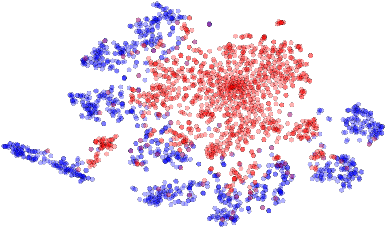
\includegraphics[width=0.45\textwidth]{./figures/adaptation_vis/pool2_mnist2inv_before.pdf}}\hfill%
  \subfigure[Adapted]{%%
    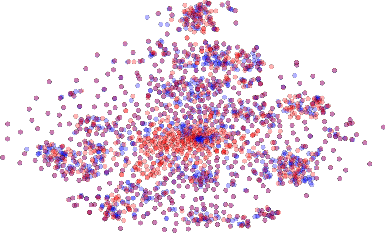
\includegraphics[width=0.45\textwidth]{./figures/adaptation_vis/pool2_mnist2inv_after.pdf}}%%
  \hspace*{\fill}%
  \end{minipage}%
  \begin{minipage}{.5\textwidth}
  \centering
  \small{{\sc Syn Numbers $ \rightarrow $ SVHN}: last hidden layer of the label predictor}
  \setcounter{subfigure}{0}
  \hspace*{\fill}%
  \subfigure[Non-adapted]{%%
    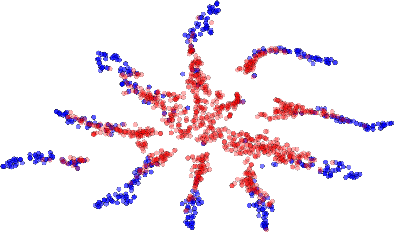
\includegraphics[width=0.45\textwidth]{./figures/adaptation_vis/before.pdf}}\hfill%
  \subfigure[Adapted]{%%
    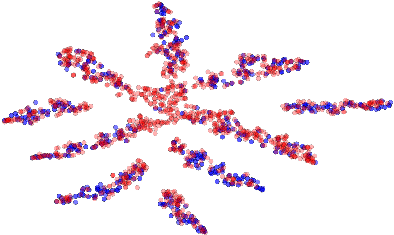
\includegraphics[width=0.45\textwidth]{./figures/adaptation_vis/after.pdf}}%%
  \hspace*{\fill}%
  \end{minipage}
  \caption{The effect of adaptation on the distribution of the extracted features (best viewed in color). The figure shows t-SNE \cite{Maaten13} visualizations of the CNN's activations {\bf (a)} in case when no adaptation was performed and {\bf (b)} in case when our adaptation procedure was incorporated into training. {\it Blue} points correspond to the source domain examples, while {\it red} ones correspond to the target domain. In all cases, the adaptation in our method makes the two distributions of features much closer.}
  \label{fig:exper_adapt_vis}
\end{figure*}

\subsection{Results}
\label{sect:exper_quant}

We now discuss the experimental settings and the results. In each case, we train on the source dataset and test on a different target domain dataset, with considerable shifts between domains (see \fig{exper_domains_examples}). The results are summarized in \tab{results} and \tab{results_office}. 

\vspace{2mm}\noindent {\bf MNIST $ \rightarrow $ MNIST-M.}
Our first experiment deals with the MNIST dataset~\cite{LeCun98} (source). In order to obtain the target domain ({\sc MNIST-M}) we blend digits from the original set over patches randomly extracted from color photos from BSDS500 \cite{Arbelaez11}. This operation is formally defined for two images $ I^{1}, I^{2} $ as $ I_{ijk}^{out} = | I_{ijk}^{1} - I_{ijk}^{2} | $, where $ i, j $ are the coordinates of a pixel and $ k $ is a channel index. In other words, an output sample is produced by taking a patch from a photo and inverting its pixels at positions corresponding to the pixels of a digit. For a human the classification task becomes only slightly harder compared to the original dataset (the digits are still clearly distinguishable) whereas for a CNN trained on MNIST this domain is quite distinct, as the background and the strokes are no longer constant. Consequently, the source-only model performs poorly. Our approach succeeded at aligning feature distributions (\fig{exper_adapt_vis}), which led to successful adaptation results (considering that the adaptation is unsupervised). At the same time, the improvement over source-only model achieved by subspace alignment (SA) \cite{Fernando13} is quite modest, thus highlighting the difficulty of the adaptation task. 

\vspace{2mm}\noindent {\bf Synthetic numbers $ \rightarrow $ SVHN.}
To address a common scenario of training on synthetic data and testing on  real data, we use Street-View House Number dataset {\sc SVHN} \cite{Netzer11} as the target domain and synthetic digits as the source. The latter ({\sc Syn ~Numbers}) consists of ~500,000 images generated by ourselves from Windows fonts by varying the text (that includes different one-, two-, and three-digit numbers), positioning, orientation, background and stroke colors, and the amount of blur. The degrees of variation were chosen manually to simulate SVHN, however the two datasets are still rather distinct, the biggest difference being the structured clutter in the background of SVHN images. 

The proposed backpropagation-based technique works well covering two thirds of the gap between training with source data only and training on target domain data with known target labels. In contrast, SA~\cite{Fernando13} does not result in any significant improvement in the classification accuracy, thus highlighting that the adaptation task is even more challenging than in the case of the MNIST experiment.

\vspace{2mm}\noindent {\bf MNIST $ \leftrightarrow $ SVHN.}
In this experiment, we further increase the gap between distributions, and test on {\sc MNIST} and {\sc SVHN}, which are significantly different in appearance. Training on SVHN even without adaptation is challenging --- classification error stays high during the first 150 epochs. In order to avoid ending up in a poor local minimum we, therefore, do not use learning rate annealing here. Obviously, the two directions ({\sc MNIST} $ \rightarrow $ {\sc SVHN} and {\sc SVHN} $ \rightarrow $ {\sc MNIST}) are not equally difficult. As {\sc SVHN} is more diverse, a model trained on SVHN is expected to be more generic and to perform reasonably on the MNIST dataset. This, indeed, turns out to be the case and is supported by the appearance of the feature distributions. We observe a quite strong separation between the domains when we feed them into the CNN trained solely on { \sc MNIST}, whereas for the {\sc SVHN}-trained network the features are much more intermixed. This difference probably explains why our method succeeded in improving the performance by adaptation in the {\sc SVHN} $ \rightarrow $ {\sc MNIST} scenario (see \tab{results}) but not in the opposite direction (SA is not able to perform adaptation in this case either). Unsupervised adaptation from MNIST to SVHN gives a failure example for our approach (we are unaware of any unsupervised DA methods capable of performing such adaptation).

\vspace{2mm}\noindent {\bf Synthetic Signs $ \rightarrow $ GTSRB.}
Overall, this setting is similar to the {\sc Syn Numbers} $ \rightarrow $ {\sc SVHN} experiment, except the distribution of the features is more complex due to the significantly larger number of classes (43 instead of 10). For the source domain we obtained~100,000 synthetic images (which we call {\sc Syn~Signs}) simulating various photoshooting conditions. Once again, our method achieves a sensible increase in performance once again proving its suitability for the synthetic-to-real data adaptation.

\begin{figure}
  \centering
  \setlength\figureheight{2.7cm}
  \setlength\figurewidth{6.8cm}
  % This file was created by matlab2tikz v0.5.0 running on MATLAB 8.3.
%Copyright (c) 2008--2014, Nico Schlömer <nico.schloemer@gmail.com>
%All rights reserved.
%Minimal pgfplots version: 1.3
%
%The latest updates can be retrieved from
%  http://www.mathworks.com/matlabcentral/fileexchange/22022-matlab2tikz
%where you can also make suggestions and rate matlab2tikz.
%
\begin{tikzpicture}[font=\scriptsize]

\begin{axis}[%
width=0.95092\figurewidth,
height=\figureheight,
at={(0\figurewidth,0\figureheight)},
scale only axis,
xmin=10000,
xmax=50000,
xlabel={Batches seen},
ymin=0,
ymax=1,
ylabel={Validation error},
axis x line*=bottom,
axis y line*=left,
legend style={at={($ (1,1) + (-0.1cm,-0.1cm) $)},anchor=north east,align=left,legend cell align=left,draw=black},
xmajorgrids,
ymajorgrids,
grid style={dashed}
]
\addplot [color=blue,solid,line width=1.0pt]
  table[row sep=crcr]{%
10500	0.199757996632997\\
11000	0.19162984006734\\
11500	0.190788089225589\\
12000	0.192918771043771\\
12500	0.196390993265993\\
13000	0.185527146464646\\
13500	0.190472432659933\\
14000	0.185606060606061\\
14500	0.183422769360269\\
15000	0.189051978114478\\
15500	0.191524621212121\\
16000	0.186079545454545\\
16500	0.179424452861953\\
17000	0.187684132996633\\
17500	0.187868265993266\\
18000	0.180923821548822\\
18500	0.187315867003367\\
19000	0.178661616161616\\
19500	0.18102904040404\\
20000	0.180555555555556\\
20500	0.176662457912458\\
21000	0.183791035353535\\
21500	0.179214015151515\\
22000	0.178898358585859\\
22500	0.178898358585859\\
23000	0.174479166666667\\
23500	0.174742213804714\\
24000	0.171059553872054\\
24500	0.177951388888889\\
25000	0.174794823232323\\
25500	0.174084595959596\\
26000	0.174636994949495\\
26500	0.169034090909091\\
27000	0.171191077441077\\
27500	0.170875420875421\\
28000	0.171506734006734\\
28500	0.170217803030303\\
29000	0.169244528619529\\
29500	0.169875841750842\\
30000	0.168744739057239\\
30500	0.17048085016835\\
31000	0.169454966329966\\
31500	0.167771464646465\\
32000	0.168849957912458\\
32500	0.168323863636364\\
33000	0.168718434343434\\
33500	0.165667087542088\\
34000	0.167376893939394\\
34500	0.169007786195286\\
35000	0.167140151515152\\
35500	0.165667087542088\\
36000	0.167850378787879\\
36500	0.169823232323232\\
37000	0.170691287878788\\
37500	0.16640361952862\\
38000	0.167981902356902\\
38500	0.169875841750842\\
39000	0.166771885521886\\
39500	0.169376052188552\\
40000	0.168087121212121\\
40500	0.165509259259259\\
41000	0.167718855218855\\
41500	0.168060816498317\\
42000	0.166035353535354\\
42500	0.166692971380471\\
43000	0.166429924242424\\
43500	0.167034932659933\\
44000	0.170349326599327\\
44500	0.169744318181818\\
45000	0.168218644781145\\
45500	0.166429924242424\\
46000	0.166324705387205\\
46500	0.168771043771044\\
47000	0.168034511784512\\
47500	0.168718434343434\\
48000	0.171059553872054\\
48500	0.170638678451178\\
49000	0.16819234006734\\
49500	0.168981481481481\\
50000	0.167902988215488\\
};
\addlegendentry{Real data only};

\addplot [color=cyan,solid,line width=1.0pt]
  table[row sep=crcr]{%
10500	0.9625\\
11000	0.79765625\\
11500	0.715625\\
12000	0.6140625\\
12500	0.52109375\\
13000	0.459375\\
13500	0.4484375\\
14000	0.421875\\
14500	0.39453125\\
15000	0.4109375\\
15500	0.34296875\\
16000	0.36875\\
16500	0.3359375\\
17000	0.36171875\\
17500	0.3171875\\
18000	0.3484375\\
18500	0.32421875\\
19000	0.315625\\
19500	0.346875\\
20000	0.31875\\
20500	0.35390625\\
21000	0.3265625\\
21500	0.33359375\\
22000	0.3171875\\
22500	0.28515625\\
23000	0.30546875\\
23500	0.309375\\
24000	0.2796875\\
24500	0.30859375\\
25000	0.30703125\\
25500	0.3078125\\
26000	0.28671875\\
26500	0.2875\\
27000	0.31484375\\
27500	0.2859375\\
28000	0.29375\\
28500	0.31328125\\
29000	0.3078125\\
29500	0.2859375\\
30000	0.2890625\\
30500	0.284375\\
31000	0.2953125\\
31500	0.26953125\\
32000	0.29921875\\
32500	0.30078125\\
33000	0.2640625\\
33500	0.309375\\
34000	0.2734375\\
34500	0.290625\\
35000	0.26796875\\
35500	0.3015625\\
36000	0.26796875\\
36500	0.2921875\\
37000	0.265625\\
37500	0.2765625\\
38000	0.2859375\\
38500	0.32109375\\
39000	0.28046875\\
39500	0.275\\
40000	0.24921875\\
40500	0.29140625\\
41000	0.26640625\\
41500	0.265625\\
42000	0.259375\\
42500	0.2765625\\
43000	0.26796875\\
43500	0.2765625\\
44000	0.27265625\\
44500	0.25546875\\
45000	0.26484375\\
45500	0.271875\\
46000	0.2703125\\
46500	0.26171875\\
47000	0.246875\\
47500	0.25078125\\
48000	0.29609375\\
48500	0.2640625\\
49000	0.26875\\
49500	0.26015625\\
50000	0.2578125\\
};
\addlegendentry{Synthetic data only};

\addplot [color=red,solid,line width=1.0pt]
  table[row sep=crcr]{%
10500	0.943892045454545\\
11000	0.943892045454545\\
11500	0.943892045454545\\
12000	0.943892045454545\\
12500	0.848300715488216\\
13000	0.658722643097643\\
13500	0.590593434343434\\
14000	0.475484006734007\\
14500	0.313946759259259\\
15000	0.235690235690236\\
15500	0.17879313973064\\
16000	0.152383207070707\\
16500	0.12912984006734\\
17000	0.114478114478114\\
17500	0.116214225589226\\
18000	0.1015625\\
18500	0.10066813973064\\
19000	0.101983375420875\\
19500	0.0914351851851852\\
20000	0.0895675505050505\\
20500	0.0894360269360269\\
21000	0.0827283249158249\\
21500	0.0798611111111111\\
22000	0.0859638047138047\\
22500	0.0799137205387205\\
23000	0.0778619528619529\\
23500	0.0737584175084175\\
24000	0.0742582070707071\\
24500	0.0776778198653199\\
25000	0.0771517255892256\\
25500	0.0725747053872054\\
26000	0.0739425505050505\\
26500	0.0734953703703704\\
27000	0.0730744949494949\\
27500	0.0688920454545455\\
28000	0.0702072811447811\\
28500	0.072337962962963\\
29000	0.0670244107744108\\
29500	0.0733638468013468\\
30000	0.0667613636363636\\
30500	0.0692340067340067\\
31000	0.0652093855218855\\
31500	0.0664720117845118\\
32000	0.0655776515151515\\
32500	0.0671296296296296\\
33000	0.0656039562289562\\
33500	0.0646043771043771\\
34000	0.0668665824915825\\
34500	0.0638678451178451\\
35000	0.065077861952862\\
35500	0.0649989478114478\\
36000	0.0672348484848485\\
36500	0.0668665824915825\\
37000	0.0626052188552189\\
37500	0.0652093855218855\\
38000	0.0626315235690236\\
38500	0.0627893518518518\\
39000	0.0613162878787879\\
39500	0.063236531986532\\
40000	0.0629208754208754\\
40500	0.0639467592592593\\
41000	0.0612899831649832\\
41500	0.0653409090909091\\
42000	0.0608691077441077\\
42500	0.0613425925925926\\
43000	0.0630260942760943\\
43500	0.060106271043771\\
44000	0.0638678451178451\\
44500	0.0602377946127946\\
45000	0.0577388468013468\\
45500	0.062684132996633\\
46000	0.0608164983164983\\
46500	0.0603167087542088\\
47000	0.0577651515151515\\
47500	0.0583175505050505\\
48000	0.0591329966329966\\
48500	0.0607112794612795\\
49000	0.0585805976430976\\
49500	0.0583175505050505\\
50000	0.0590540824915825\\
};
\addlegendentry{Both};

\end{axis}
\end{tikzpicture}%
  \caption{Semi-supervised domain adaptation for the traffic signs. As labeled target domain data are shown to the method, it achieves significantly lower error than the model trained on target domain data only or on source domain data only. \vspace{-4mm}}
  \label{fig:exper_semi_test}
\end{figure}

As an additional experiment, we also evaluate the proposed algorithm for semi-supervised domain adaptation, i.e.\ when one is additionally provided with a small amount of labeled target data. For that purpose we split {\sc GTSRB} into the train set (1280 random samples with labels) and the validation set (the rest of the dataset). The validation part is used solely for the evaluation and does not participate in the adaptation. The training procedure changes slightly as the label predictor is now exposed to the target data. \fig{exper_semi_test} shows the change of the validation error throughout the training. While the graph clearly suggests that our method can be used in the semi-supervised setting, thorough verification of semi-supervised setting is left for future work.


\vspace{2mm}\noindent {\bf Office dataset.} 
We finally evaluate our method on {\sc Office} dataset, which is a collection of three distinct domains: {\sc Amazon}, {\sc DSLR}, and {\sc Webcam}. Unlike previously discussed datasets, {\sc Office} is rather small-scale with only 2817 labeled images spread across 31 different categories in the largest domain. The amount of available data is crucial for a successful training of a deep model, hence we opted for the fine-tuning of the CNN pre-trained on the ImageNet \cite{Jia14} as it is done in some recent DA works \cite{Donahue14,Tzeng14,Hoffman14}. We make our approach more comparable with \cite{Tzeng14} by using exactly the same network architecture replacing domain mean-based regularization with the domain classifier.

Following most previous works, we evaluate our method using 5 random splits for each of the 3 transfer tasks commonly used for evaluation. Our training protocol is close to \cite{Tzeng14,Saenko10,Gong12} as we use the same number of labeled source-domain images per category. Unlike those works and similarly to e.g.\ DLID~\cite{Chopra13} we use the whole unlabeled target domain (as the premise of our method is the abundance of unlabeled data in the target domain). Under this transductive setting, our method is able to improve previously-reported state-of-the-art accuracy for unsupervised adaptation very considerably (\tab{results_office}), especially in the most challenging {\sc Amazon} $ \rightarrow $ {\sc Webcam} scenario (the two domains with the largest domain shift).


\section{Related Work}
\section{Related work}\label{s:related}

\begin{figure}[t]
\centering
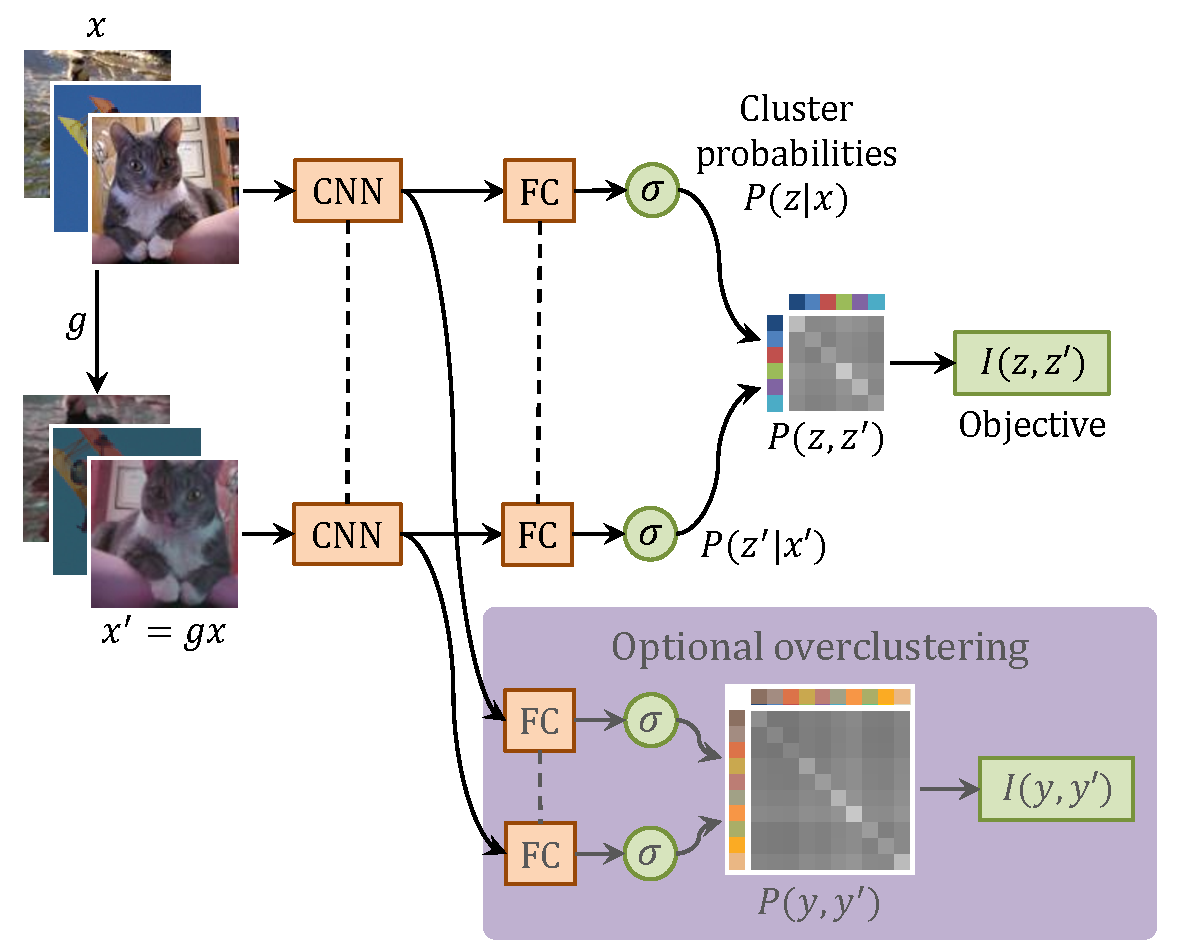
\includegraphics[width=0.95\columnwidth]{paper_imgs/overview1.pdf}
\caption{\label{f:overview}\methodnameshort for image clustering. Dashed line denotes shared parameters, $g$ is a random transformation, and $I$ denotes mutual information~(\cref{e:loss_expanded}).}
\end{figure}


\begin{figure*}
%\captionsetup{justification=centering}
\setlength\tabcolsep{2.2pt} % default value: 6pt

\begin{tabular}{c c c c c c}
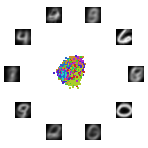
\includegraphics[height=0.16\textwidth]{experiments2_files/mnist_progression/726_run_1_colour_0_pointcloud_0.png} & 
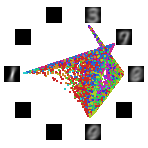
\includegraphics[height=0.16\textwidth]{experiments2_files/mnist_progression/726_run_1_colour_0_pointcloud_3.png} & 
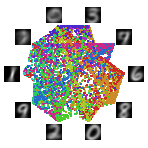
\includegraphics[height=0.16\textwidth]{experiments2_files/mnist_progression/726_run_1_colour_0_pointcloud_10.png} & 
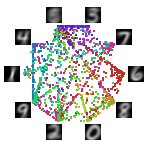
\includegraphics[height=0.16\textwidth]{experiments2_files/mnist_progression/726_run_1_colour_0_pointcloud_30.png} & 
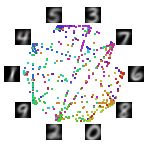
\includegraphics[height=0.16\textwidth]{experiments2_files/mnist_progression/726_run_1_colour_0_pointcloud_101.png} & 
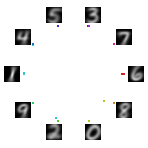
\includegraphics[height=0.16\textwidth]{experiments2_files/mnist_progression/726_run_1_colour_0_pointcloud_1000.png} 
\end{tabular}

\caption{\label{f:mnist_dots} Training with \methodnameshort on unlabelled MNIST in successive epochs from random initialisation (left). The network directly outputs cluster assignment probabilities for input images, and each is rendered as a coordinate by convex combination of 10 cluster vertices. There is no cherry-picking as the entire dataset is shown in every snapshot. Ground truth labelling (unseen by model) is given by colour. At each cluster the average image of its assignees is shown. With neither labels nor heuristics, the clusters discovered by \methodnameshort correspond perfectly to unique digits, with one-hot certain prediction (right).}
\end{figure*}


\paragraph{Co-clustering and mutual information.}

The use of information as a criterion to learn representations is not new. One of the earliest works to do so is by Becker and Hinton~\cite{becker1992self}.
More generally, learning from paired data has been explored in co-clustering~\cite{hartigan1972direct, dhillon2003information} and in other works~\cite{wang2010information} that build on the information bottleneck principle~\cite{friedman2001multivariate}.

Several recent papers have used information as a tool to train deep networks in particular.
IMSAT~\cite{hu2017learning} maximises mutual information between data and its representation and DeepINFOMAX~\cite{hjelm2018learning} maximizes information between spatially-preserved features and compact features.
However, IMSAT and DeepINFOMAX combine information with other criteria, whereas in our method information is the only criterion used.
Furthermore, both IMSAT and DeepINFOMAX compute mutual information over continuous random variables, which requires complex estimators~\cite{belghazi2018mine}, whereas \methodnameshort does so for discrete variables with simple and exact computations.
Finally, DeepINFOMAX considers the information $I(\bx, f(\bx))$ between the features $\bx$ and a deterministic function $f(\bx)$ of it, which is in principle the same as the entropy $H(\bx)$; in contrast, in \methodnameshort information does not trivially reduce to  entropy.

\paragraph{Semantic clustering versus intermediate representation learning.}
In semantic clustering, the learned function directly outputs discrete assignments for high level (i.e. semantic) clusters. Intermediate representation learners, on the other hand, produce continuous, distributed, high-dimensional representations that must be post-processed, for example by k-means, to obtain the discrete low-cardinality assignments required for unsupervised semantic clustering. The latter includes objectives such as generative autoencoder image reconstruction~\cite{vincent2010stacked},  triplets~\cite{schultz2004learning} and spatial-temporal order or context prediction~\cite{lee2017unsupervised,cruz2017deeppermnet,doersch2015unsupervised}, for example predicting patch proximity~\cite{isola2015learning}, solving jigsaw puzzles~\cite{noroozi2016unsupervised} and inpainting~\cite{pathak2016context}. Note it also includes a number of clustering methods (DeepCluster~\cite{caron2018deep}, exemplars~\cite{dosovitskiy2015discriminative}) where the clustering is only auxiliary; a clustering-style objective is used but does not produce groups with semantic correspondence. For example, DeepCluster~\cite{caron2018deep} is a state-of-the-art method for learning highly-transferable intermediate features using overclustering as a proxy task, but does not automatically find semantically meaningful clusters. As these methods use auxiliary objectives divorced from the semantic clustering objective, it is unsurprising that they perform worse than \methodnameshort~(\cref{s:experiments}), which directly optimises for it, training the network end-to-end with the final clusterer implicitly wrapped inside.




\paragraph{Optimising image-to-image distance.}

Many approaches to deep clustering, whether semantic or auxiliary, utilise a distance function between input images that approximates a given grouping criterion.
Agglomerative clustering~\cite{bautista2016cliquecnn} and partially ordered sets~\cite{bautista2017deep} of HOG features~\cite{dalal2005histograms} have been used to group images, and exemplars~\cite{dosovitskiy2015discriminative} define a group as a set of random transformations applied to a single image. Note the latter does not scale easily, in particular to image segmentation where a single $200\times 200$ image would call for 40k classes. DAC~\cite{chang2017deep}, JULE~\cite{yang2016joint}, DeepCluster~\cite{caron2018deep}, ADC~\cite{haeusser2018associative} and DEC~\cite{xie2016unsupervised} rely on the inherent visual consistency and disentangling properties~\cite{greff2015binding} of CNNs to produce cluster assignments, which are processed and reinforced in each iteration. 
The latter three are based on k-means style mechanisms to refine feature centroids, which is prone to degenerate solutions~\cite{caron2018deep} and thus needs explicit prevention mechanisms such as pre-training, cluster-reassignment or feature cleaning via PCA and whitening~\cite{xie2016unsupervised, caron2018deep}.

\begin{comment}
DAC is the only unsupervised clustering algorithm out of these that eschews k-means and agglomerative clustering for a different but similar clustering scheme, based on feature inner-products rather than distances.
DAC forms clusters gradually, in a self-paced manner, thus alleviating but not eliminating the risk of incurring degenerate solutions.
Furthermore, the nature of the optimisation, which reinforces bootstrapped class labels, creates a strong dependency on initialisation.

For unsupervised feature learning in general, i.e.\ where the training objective is not clustering, a large number of works explore using proxy learning tasks. 
There are two major directions:  generative tasks such as autoencoder image reconstruction~\cite{vincent2010stacked}, and spatial-temporal order or context prediction~\cite{lee2017unsupervised,cruz2017deeppermnet,doersch2015unsupervised}. The latter includes predicting patch proximity~\cite{isola2015learning}, solving jigsaw puzzles~\cite{noroozi2016unsupervised} and inpainting~\cite{pathak2016context}. 
In many cases they benefit from principled formulations that protect against degeneracy.
However, unlike the aforementioned clustering methods, the features learned by these methods need to be post-processed, for example using k-means, to cluster the data. 

\end{comment}

\paragraph{Invariance as a training objective.}

Optimising for function outputs to be persistent through spatio-temporal or non-material distortion is an idea shared by \methodnameshort with several works, including exemplars~\cite{dosovitskiy2015discriminative}, IMSAT~\cite{hu2017learning}, proximity prediction~\cite{isola2015learning}, the denoising objective of Tagger~\cite{greff2016tagger}, temporal slowness constraints~\cite{zou2012deep}, and optimising for features to be invariant to local image transformations~\cite{sohn2012learning,hui2013direct}.
More broadly, the problem of modelling data transformation has received significant attention in deep learning, one example being the transforming autoencoder~\cite{hinton2011transforming}.


% \section{Related work}\label{s:related}

% \paragraph{Co-clustering and mutual information.}

% The idea of learning a data representation by seeking the common parts of related observations is not new. 
% An early work is Becker and Hinton~\cite{becker1992self}, which maximises agreement between representations of 2D images to learn depth, using an objective corresponding to maximising mutual information between the input and the average of the data representations. 
% Co-learning has also been explored in the context of clustering by co-clustering methods, dating back to the pioneering work of Hartigan~\cite{hartigan72direct}. 
% Many information-theoretic variant of such approaches have been proposed, as discussed by~\cite{wang10information}, which are generally related to the information bottleneck principle~(\cite{friedman2001multivariate}). 

% A few works have employed mutual information in the context of unsupervised deep learning. IMSAT~\cite{hu2017learning} maximises mutual information between input data and their predicted discrete representations whilst encouraging the representations of augmented data points to be close to those of the original data points. 
% DeepINFOMAX~\cite{hjelm2018learning} maximises mutual information between spatially preserved features and compact features. There are some major differences with \methodnameshort. 
% Firstly, mutual information is used as an aid in these methods, as it increases the statistical predictivity between two random variables. 
% This contrasts with our method, where mutual information constitutes the loss applied directly to cluster assignments, meaning it is used as a clustering objective. 
% Secondly, both IMSAT and DeepINFOMAX compute mutual information over continuous random variables, which calls for an integral and is not computationally tractable, so estimators~\cite{belghazi2018mine} are used. 
% Since \methodnameshort maximises mutual information between cluster assignments and the number of clusters is discrete, computation is exact and straightforward. 
% Finally, DeepINFOMAX employs mutual information between function inputs and outputs, i.e. $I(x, f(x))$, but the conditional entropy component of mutual information $H(f(x) | x)$ is 0 when $f$ is deterministic, making the maximisation less meaningful. 
% In contrast \methodnameshort maximises mutual information between cluster assignments of separate images, i.e. $I(z, z')$ where $z$ and $z'$ are not functions of one other, making $H(z | z')$ a non-zero quantity that contributes to the optimisation as it can be minimised.

% \paragraph{Optimising image-to-image distance for clustering.}
% Many works for on unsupervised deep clustering involve establishing a scheme for estimating the semantic distance between input images, before training a function to learn this scheme. 
% CliqueCNN~\cite{bautista2016cliquecnn} trains a network to discriminate between cliques that are determined by applying agglomerative clustering on image features such as HOG~\cite{dalal2005histograms}. 
% In Exemplar CNNs~\cite{dosovitskiy2016discriminative}, each image and a its set of random transformations is considered a class, and a function is trained to discriminate between these surrogate classes. Like \methodnameshort, this method uses random transformations as a proxy for obtaining images with low semantic distance in the absence of label information. 
% Requiring one class per input image has a large memory footprint which makes Exemplar CNNs infeasible for segmentation (where patches are clustered instead of images, so a single 200x200 image would call for 40k classes). 

% \begin{figure}[t]
\centering
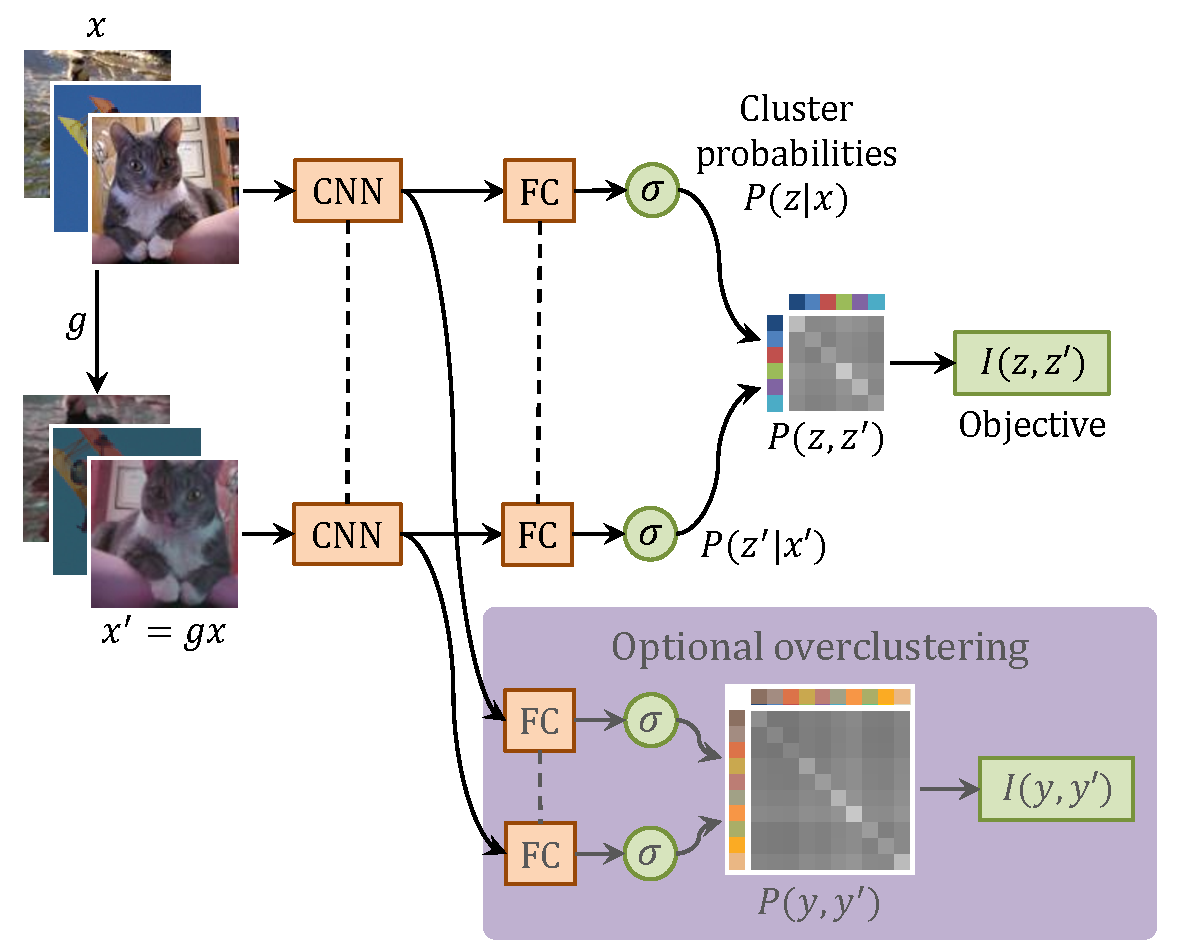
\includegraphics[width=0.95\columnwidth]{paper_imgs/overview1.pdf}
\caption{\label{f:overview}\methodnameshort for image clustering. Dashed line denotes shared parameters, $g$ is a random transformation, and $I$ denotes mutual information~(\cref{e:loss_expanded}).}
\end{figure}


% DAC~\cite{chang2017deep}, JULE~\cite{yang2016joint}, DeepCluster~\cite{caron2018deep}, Associative Deep Clustering~\cite{haeusser18associative} and DEC~\cite{xie2016unsupervised} all rely on the inherent visual consistency and disentangling properties~\cite{greff2015binding} of CNNs to produce meaningful cluster assignments, which are processed and reinforced in each iteration. 
% The latter three are based on using k-means to refine deep feature vectors, a mechanism which is prone to degenerate solutions~\cite{caron2018deep} and thus needs explicit prevention mechanisms such as pre-training, cluster-reassignment or feature cleaning via PCA and whitening ~\cite{xie2016unsupervised, caron2018deep}. 

% DAC is the only unsupervised clustering algorithm out of these that eschews k-means whilst training a network to directly produce cluster assignments, as \methodnameshort does. 
% A network is trained to produce cluster assignment probability distributions for each sample that are used as high level feature descriptors, and the dot product of different descriptors is treated as a proxy for inter-sample semantic distance (instead of Euclidian distance, which is used in the k-means based clusterers). 
% Training proceeds by maximising the dot product of close sample pairs, thus encouraging them to be assigned to the same cluster, whilst minimising the dot product for far pairs. 
% The nature of the optimisation means there is a strong dependency on initialisation and lack of protection against degenerate solutions such as clusters disappearing. 

% \paragraph{Proxy tasks for unsupervised feature learning.}
% For unsupervised feature learning in general, i.e. where the training objective is not clustering, a large number of works explore using proxy learning tasks. 
% There are two major camps:  generative tasks such as autoencoder image reconstruction~\cite{vincent2010stacked}, and spatial-temporal order or context prediction~\cite{lee2017unsupervised,cruz2017deeppermnet,doersch2015unsupervised}. The latter includes predicting patch proximity~\cite{isola2015learning}, solving jigsaw puzzles~(\cite{noroozi2016unsupervised}) and inpainting~(\cite{pathak2016context}). 
% In many cases they benefit from principled formulations that protect against degeneracy.
% However, unlike the aforementioned clustering methods, learned representations from these tasks constitute fine-grained continuous features rather than coarse cluster assignments, and thus must be post-processed, either by unsupervised clustering such as k-means or with label information via SVMs or fine-tuning, in order to produce semantic clusters.

% \paragraph{Invariance as a training objective.}
% Training for function outputs to be persistent through spatio-temporal distortion, noise distortion, or random transforms is an idea shared by \methodnameshort and several mentioned works, including Exemplar CNNs~\cite{dosovitskiy2016discriminative}, IMSAT~\cite{hu2017learning} and proximity prediction~\cite{isola2015learning}.
% It is also seen in Tagger~\cite{greff2016tagger}, which trains a function to denoise its input using several clusters to distribute the representation,~\cite{zou2012deep} which enforces a temporal slowness constraint on learned features, and~\cite{sohn2012learning,hui2013direct} which train for features invariant to local image transformations.




\section{Conclusion}
\label{sec:conclusion}
We introduce a novel neural network architecture, the Synchronized Spectral CNN (SyncSpecCNN), for semantic annotation on 3D shape graphs. To share coefficients and conduct multi-scale analysis in different parts of a single shape graph, we introduce a spectral parametrization of dilated convolutional kernels. To allow parameter sharing across related but different shapes that may be represented by very different graphs, we introduce a spectral transformer network to synchronize different spectral domains. The effectiveness of different components in our network is validated through extensive experiments. Jointly these contributions lead to state-of-the-art performance on various semantic annotation tasks including 3D shape part segmentation and 3D keypoint prediction.


%\subsubsection*{Acknowledgments}

\bibliography{bibliography}
\bibliographystyle{iclr2016_conference}

\newpage
\appendix

\section{Discrimination metrics}
The Discrimination metric~\citep{zemel2013learning} and the Discrimination metric that takes into account the probabilities of the correct class are mathematically formalized as:
 
\begin{align*}
 \text{Discrimination} & = \bigg|\frac{\sum_{n=1}^{N}\mathbb{I}[y_n^{s=0}]}{N_{s = 0}} - \frac{\sum_{n=1}^{N}\mathbb{I}[y_n^{s=1}]}{N_{s=1}}\bigg| \\  
  \text{Discrimination prob.} & = \bigg|\frac{\sum_{n=1}^{N}p(y_n^{s=0})}{N_{s = 0}} - \frac{\sum_{n=1}^{N}p(y_n^{s=1})}{N_{s=1}}\bigg|
\end{align*}
where $\mathbb{I}[y_n^{s=0}] = 1$ for the predictions $y_n$ that were done on the datapoints with nuisance variable $s = 0$, $N_{s=0}$ denotes the total amount of datapoints that had nuisance variable $s = 0$ and $p(y_n^{s=0})$ denotes the probability of the prediction $y_n$ for the datapoints with $s=0$. For the predictions and their respective probabilities we used a Logistic Regression classifier.

\section{Proxy A-Distance (PAD) for Amazon Reviews dataset}
Similarly to~\cite{2015arXiv150507818G}, we also calculated the Proxy A-distance (PAD)~\citep{ben2007analysis,ben2010theory} scores for the raw data $\*x$ and for the $\*z_1$ representations of VFAE. Briefly, Proxy A-distance is an approximation to the $\mathcal{H}$-divergence measure of domain distinguishability proposed in~\cite{kifer2004detecting} and~\cite{ben2007analysis,ben2010theory}. To compute it we first need to train a learning algorithm on the task of discriminating examples from the source and target domain. Afterwards we can use the test error $\epsilon$ of that algorithm in the following formula:
\begin{align*}
  \text{PAD}(\epsilon)  = 2(1 - 2\epsilon) 
\end{align*}
It is clear that low PAD scores correspond to low discrimination of the source and target domain examples from the classifier. To obtain $\epsilon$ for our model we used Logistic Regression. The resulting plot can be seen in Figure~\ref{fig:pad_reviews}, where we have also added the plot from DANN~\citep{2015arXiv150507818G}, where they used a linear Support Vector Machine for the classifier, as a reference. It can be seen that our VFAE model can factor out the information about $\*s$ better, since the PAD scores on our new representation are, overall, lower than the ones obtained from the DANN architecture.

\begin{figure}[ht]
    \centering
    \begin{subfigure}{.49\textwidth}
    \centering
        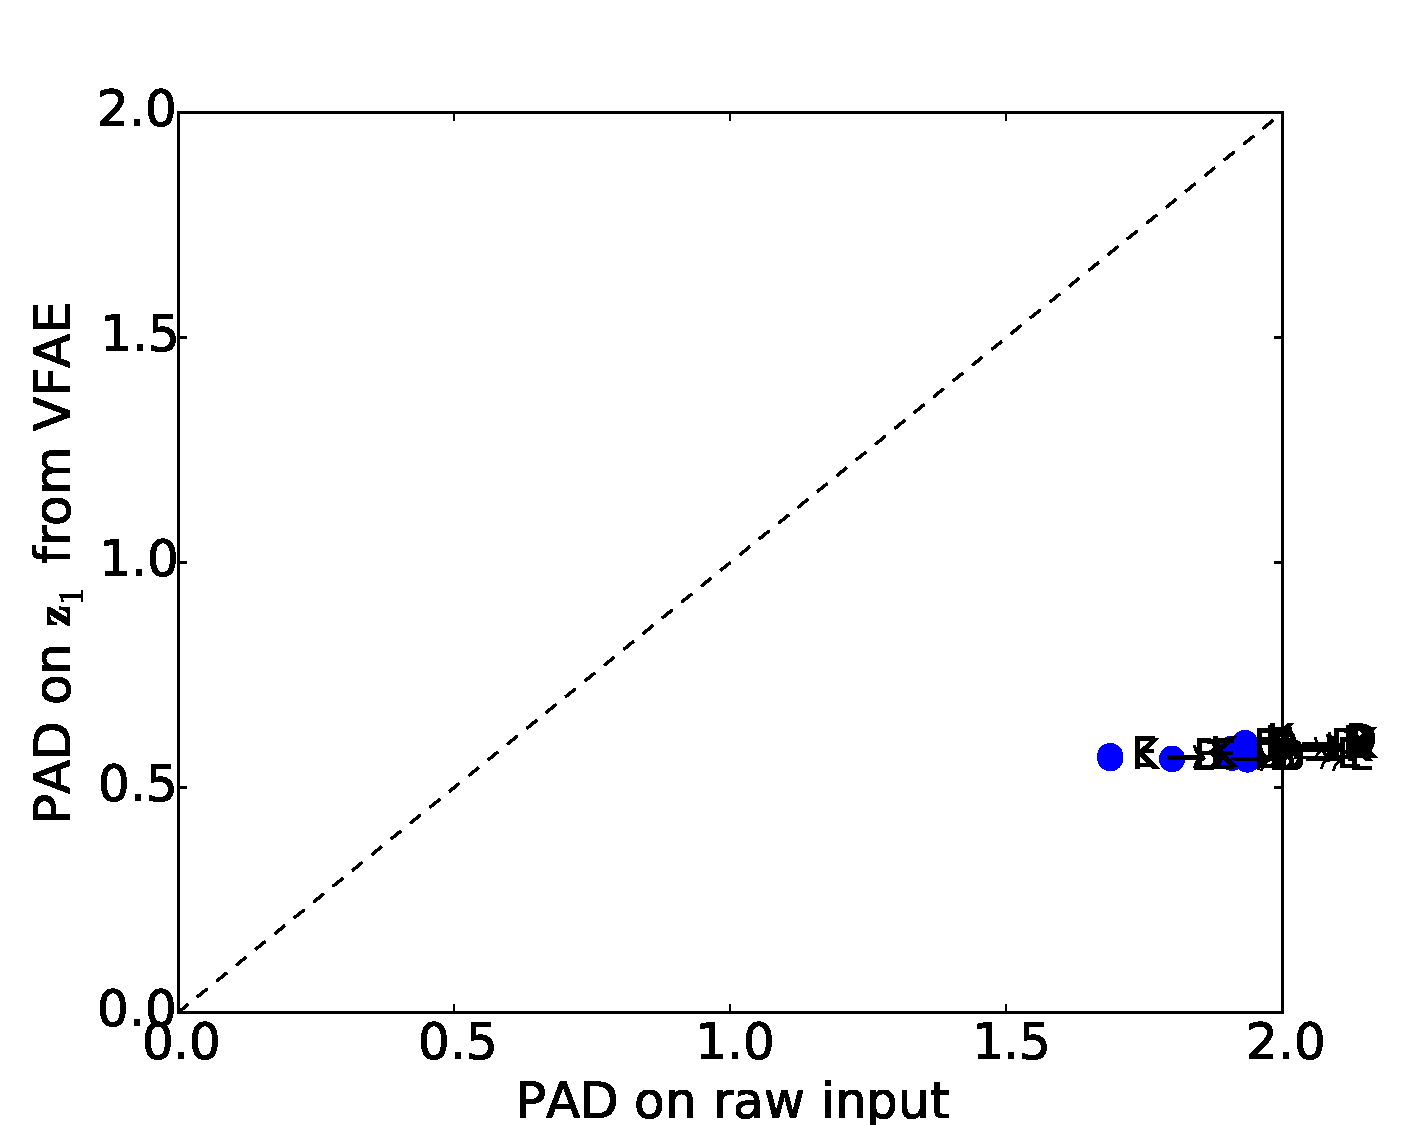
\includegraphics[width=1.\textwidth]{pad_vfae_x_reviews.pdf}
  \end{subfigure} %
    \begin{subfigure}{.49\textwidth}
      \centering
        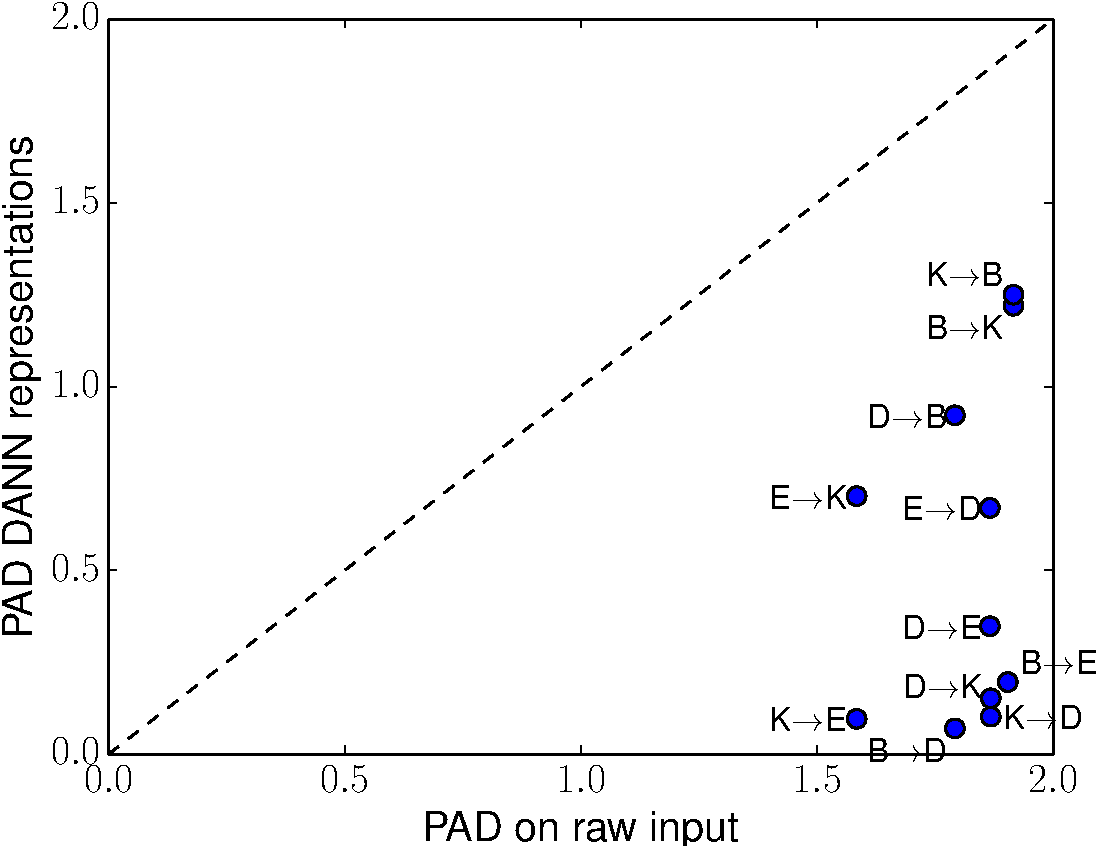
\includegraphics[width=.9\textwidth]{PAD_DANN.pdf}
     \end{subfigure} % 
    \caption{Proxy A-distances (PAD) for the Amazon reviews dataset: left from our VFAE model, right from the DANN model (taken from~\cite{2015arXiv150507818G})}
    \label{fig:pad_reviews}
\end{figure}

\end{document}
